\documentclass[]{politex}
% ========== Opções ==========
% pnumromarab - Numeração de páginas usando algarismos romanos na parte pré-textual e arábicos na parte textual
% abnttoc - Forçar paginação no sumário conforme ABNT (inclui "p." na frente das páginas)
% normalnum - Numeração contínua de figuras e tabelas 
%	(caso contrário, a numeração é reiniciada a cada capítulo)
% draftprint - Ajusta as margens para impressão de rascunhos
%	(reduz a margem interna)
% twosideprint - Ajusta as margens para impressão frente e verso
% capsec - Forçar letras maiúsculas no título das seções
% espacosimples - Documento usando espaçamento simples
% espacoduplo - Documento usando espaçamento duplo
%	(o padrão é usar espaçamento 1.5)
% times - Tenta usar a fonte Times New Roman para o corpo do texto
% noindentfirst - Não indenta o primeiro parágrafo dos capítulos/seções


% ========== Packages ==========
\usepackage[utf8]{inputenc}
\usepackage{amsmath,amsthm,amsfonts,amssymb}
\usepackage{graphicx,cite,enumerate}

\usepackage{multicol}
\usepackage{color}
\usepackage{empheq}
\usepackage{scalerel}
\usepackage{accents}
\usepackage{special-char}
\usepackage{fancybox}

\definecolor{myblue}{rgb}{.75, .75, 1}
\newcommand*\mybluebox[1]{%
\colorbox{myblue}{\hspace{1em}#1\hspace{1em}}}

\definecolor{lightblue}{rgb}{.9, .9, 1}
\newcommand*\lightbluebox[1]{%
\colorbox{lightblue}{\hspace{1em}#1\hspace{1em}}}

\definecolor{corn}{rgb}{0.98, 0.93, 0.36}
\newcommand*\cornbox[1]{%
\colorbox{corn}{\hspace{1em}#1\hspace{1em}}}

\definecolor{myyellow}{rgb}{1.0, 1.0, 0.7}
\newcommand*\myyellowbox[1]{%
\colorbox{myyellow}{\hspace{1em}#1\hspace{1em}}}

\definecolor{almond}{rgb}{0.94, 0.89, 0.82}
\newcommand*\almondbox[1]{%
\colorbox{almond}{\hspace{1em}#1\hspace{1em}}}


% ========== Language options ==========
\usepackage[brazil]{babel}
%\usepackage[english]{babel}


% ========== ABNT (requer ABNTeX 2) ==========
%	http://www.ctan.org/tex-archive/macros/latex/contrib/abntex2
\usepackage[num]{abntex2cite}

% Forçar o abntex2 a usar [ ] nas referências ao invés de ( )
\citebrackets{[}{]}


% ========== Lorem ipsum ==========
\usepackage{blindtext}



% ========== Opções do documento ==========
% Título
\titulo{Simulação dinâmica e validação experimental de técnicas de controle para manipuladores paralelos}

% Autor
\autor{André Garnier Coutinho}

% Para múltiplos autores (TCC)
%\autor{Nome Sobrenome\\%
%		Nome Sobrenome\\%
%		Nome Sobrenome}

% Orientador / Coorientador
\orientador{Prof. Dr. Tarcisio Antonio Hess Coelho}
%\coorientador{Nome do coorientador (opcional)}

% Tipo de documento
%\tcc{Eletricista com ênfase em Sistemas Eletrônicos}
%\dissertacao{Engenharia Elétrica}
\teseDOC{Engenharia Mecânica}
%\teseLD
%\memorialLD

% Departamento e área de concentração
\departamento{PMR – Eng. Mecatrônica e de Sistemas Mecânicos}
\areaConcentracao{Engenharia Mecânica de Projeto e Fabricação}

% Local
\local{São Paulo}

% Ano
\data{2019}




\begin{document}

\setcounter{MaxMatrixCols}{50}

% ========== Capa e folhas de rosto ==========
\capa
\falsafolhaderosto
\folhaderosto


% ========== Folha de assinaturas (opcional) ==========
\begin{folhadeaprovacao}
	\assinatura{Prof. Dr. Tarcisio Antonio Hess Coelho}
	\assinatura{Prof. Dr. Renato Maia Matarazzo Orsino}
	\assinatura{Profª. Dra. Maira Martins da Silva}
	\assinatura{Prof. Dr. Bruno Augusto Angélico}
	\assinatura{Prof. Dr. Diego Colón}
\end{folhadeaprovacao}


% ========== Ficha catalográfica ==========
% Fazer solicitação no site:
%	http://www.poli.usp.br/en/bibliotecas/servicos/catalogacao-na-publicacao.html


% ========== Dedicatória (opcional) ==========
%\dedicatoria{Dedicatória}


% ========== Agradecimentos ==========
\begin{agradecimentos}

Gostaria de agradecer a todos que sempre me apoiaram e ajudaram a perseguir o meu sonho de me tornar Doutor em Engenharia Mecânica pela Escola Politécnia da USP. Não tenho palavras para descrever o que significa para mim poder estar contribuindo ativamente na exploração das fronteiras do conhecimento.

Dentre as várias pessoas que sempre estiveram ao lado nesta jornada, gostaria de destacar o meu orientador e amigo Prof. Dr. Tarcisio Antonio Hess Coelho, o qual sempre esteve ao meu lado desde o início da jornada no meio acadêmico, sempre sendo super solícito, me apoiando, e me orientando da melhor maneira possível; meu grande amigo Prof. Dr. Renato Maia Matarazzo Orsino, o qual me introduziu e ensinou o que há de mais sofisticado e eficiente na parte de modelagem de sistemas multicorpos, um conhecimento fundamental para o desenvolvimento desta tese, também sempre sendo extremamente solícito e me ajudando sempre que podia; aos grandes amigos Engª. Juliana Martins de Oliveira Fuess e Eng. Victor Pacheco Bartholomeu, os quais participaram ativamente e possibilitaram o desenvolvimento do protótipo de manipulador paralelo que possibilitou adicionar um caráter experimental na tese desenvolvida; à minha namorada Adriana Marques Cavalcanti, a qual está há mais de 12 anos ao meu lado, sempre me apoiando em todos os momentos e me inspirando a ser cada vez mais uma pessoa melhor; e aos meus pais Antonio Valdec Martins Coutinho e Taïs Borges Garnier, e avó Maria Luiza Borges Garnier, os quais estão sempre se preocuparam muito comigo, sempre me apoiando e ajudando de todas as maneiras.

Por último, mas não menos importante, além dessas pessoas incríveis que tive a oportunidade de conhecer em minha vida, gostaria de destacar meu agradecimento a outras três pessoas maravilhosas que conheci há pouco tempo, que mudaram minha vida, e que tornaram possível a conclusão desta tese de doutorado: minha psicóloga Dra. Ana Maria Canzonieri, minha psiquiatra Dra. Letícia Pacheco Lessa, e minha professora de yoga Alessandra Dotto.

Muito obrigado a todos, sem vocês nada disso seria possível.

\end{agradecimentos}


% ========== Epígrafe (opcional) ==========
\epigrafe{%
	\emph{`` `Nesta direção', disse o Gato, girando a pata direita, `mora um Chapeleiro. E nesta direção', apontando com a pata esquerda, `mora uma Lebre de Março. Visite quem você quiser, são ambos loucos.' \\
	`Mas eu não ando com loucos', observou Alice. \\
	`Oh, você não tem como evitar', disse o Gato, `somos todos loucos por aqui. Eu sou louco. Você é louca'. \\
	`Como é que você sabe que eu sou louca?', disse Alice. \\
	`Você deve ser', disse o Gato, `Senão não teria vindo para cá.' ''}
	\begin{flushright}
		-{}- Lewis Carroll
	\end{flushright}
}


% ========== Resumo ==========
\begin{resumo}
Para realizar o projeto de um sistema de controle, em geral, \'e necess\'ario primeiramente de um modelo da planta a ser controlada. O grau de fidelidade do modelo da planta, dentro das condi\c{c}\~oes de opera\c{c}\~ao desejadas do sistema, influi diretamente no desempenho do sistema em malha fechada que o projeto do controlador pode oferecer. Quanto mais rico for o modelo, mais f\'acil de atingir requisitos de desempenho mais elevados (menor tempo de resposta e menor sobressinal, por exemplo) garantindo a estabilidade do sistema.

Utilizando os m\'etodos tradicionais de modelagem de Sistemas Mec\^anicos Multicorpos, \'e dif\'icil e trabalhoso de se obter modelos de sistemas complexos, como mecanismos paralelos. Para contornar esse problema, \'e comum desprezar alguns efeitos de acoplamentos inerciais, simplificando o processo de modelagem. Por\'em, essa estrat\'egia gera modelos mais pobres, o que ir\'a limitar o desempenho que o sistema poder\'a atingir quando for feito o projeto do sistema de controle.

A solu\c{c}\~ao proposta para ser poss\'ivel aumentar o desempenho, garantindo a robustez, de um sistema de controle de mecanismos paralelos \'e a utiliza\c{c}\~ao dos novos m\'etodos e estratégias de modelagem din\^amica desenvolvidos pelo grupo de pesquisa do Prof. Doutor Tarcisio Antonio Hess Coelho, os quais s\~ao adequados para incluir todos os efeitos da din\^amica de corpos r\'igidos, independentemente da complexidade do sistema.

A presente tese visa desenvolver um algoritmo de modelagem que inclua todos os efeitos da din\^amica de corpos r\'igidos para realizar a modelagem din\^amica de mecanismos paralelos (baseado na metodologia Orsino), desenvolver uma metodologias de projeto de controle robusto para mecanismos paralelos tradicionais e mecanismos com atua\c{c}\~ao redundante, e realizar simulações e valida\c{c}\~oes experimentais das leis de controle sintetizadas pela metodologia proposta.
%
\\[3\baselineskip]
%
\textbf{Palavras-Chave} -- Mecanismos paralelos, Robótica, Modelagem Dinâmica , Controle, Controle não linear.
\end{resumo}


% ========== Abstract ==========
\begin{abstract}
Abstract...
%
\\[3\baselineskip]
%
\textbf{Keywords} -- Word, Word, Word, Word, Word.
\end{abstract}


% ========== Listas (opcional) ==========
\listadefiguras
\listadetabelas

% ========== Sumário ==========
\sumario



% ========== Elementos textuais ==========

\part{Introdução}
	
\chapter{Introdução}
\capepigrafe[0.5\textwidth]{``Frase espirituosa de um autor famoso''}{Autor famoso}

Os mecanismos de arquitetura paralela são amplamente utilizados em simuladores de voo, simuladores automobilisticos, e tarefas de {\em pick-and-place}. Além disso, também são empregados em sistemas de posicionamento, sistemas de medição, máquinas de usinagem, entre outras tarefas. 

Há uma série de vantagens em utilizar mecanismos paralelos no lugar dos tradicionais seriais. Dentre elas podemos citar sua grande capacidade de carga, alta precisão de posicionamento, alta rigidez estrutural, e uma redução significativa na inércia \cite{Cheng, Khalil, Merlet2002, Tsai}. Outra característica marcante desse tipo de arquitetura são as altas velocidades e acelerações atingidas, as quais superam muito os valores máximos atingidos utilizando arquitetura serial. Grande parte dessas vantagens se devem à possibilidade de instalação de todos os motores na base imóvel do mecanismo. Como desvantagens podemos citar o menor espaço de trabalho e modelo dinâmico muito mais complexo e de difícil obtenção \cite{Rynaldo, Merlet2002}.

\begin{figure}[h!]
	\centering
	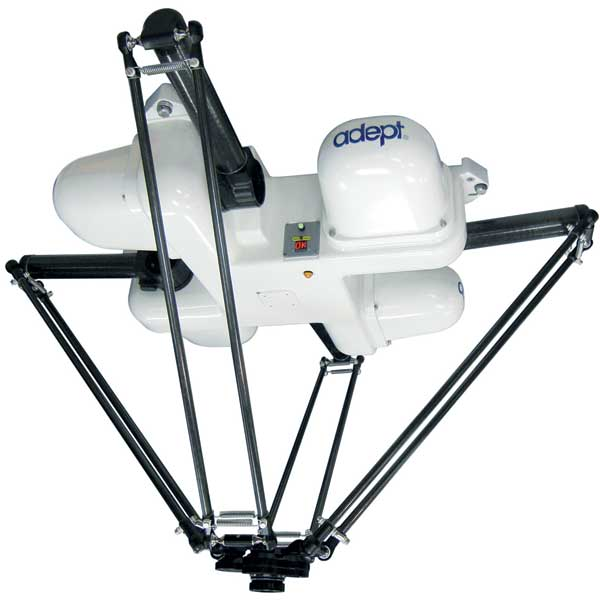
\includegraphics[scale=0.17]{../figures/theadeptquat.jpg}  
	\caption{Robô industrial Adept Quattro}
	\label{fig:Mecanismo}
\end{figure}

Levando-se em conta esta dificuldade de obtenção e a complexidade inerente do modelo dinâmico, o controle de mecanismos de arquitetura paralela é uma tarefa desafiadora. A utilização de modelos dinâmicos simplificados limita o desempenho do projeto de controladores baseados no modelo. Porém, mesmo na hipótese do modelo dinâmico completo estar disponível, o emprego de técnicas de controle não linear pode acarretar um custo  computacional muito elevado \cite{Craig, Slotini, Zubizarreta}. Este paradigma, aliado à falta de estratégias de controle apropriadas para esse tipo de mecanismos, resulta na exploração insatisfatória dos potenciais promissores de tais máquinas, como resposta dinâmica rápida e alta precisão \cite{Abdellatif}. Além disso, observa-se na literatura a escassez de trabalhos publicados com comprovação experimental de técnicas de controle aplicáveis a mecanismos paralelos \cite{Rynaldo}.
	
    Uma alternativa para a superação desta dificuldade seria a combinação de técnicas de controle não linear robusto (por exemplo, controle por modos deslizantes \cite{Slotini, Utkin}) com modelos dinâmicos completos de mecanismos paralelos, desenvolvidos a partir de novas metodologias de modelagem de sistemas multicorpos \cite{22orsino, Orsino2013, 23orsino, 21orsino}. Com esta estratégia, torna-se possível sintetizar leis de controle de alto desempenho e custo computacional mais adequado, viabilizando a exploração do potencial promissor dos mecanismos paralelos.

%OBJETIVOS E JUSTIFICATIVAS--------------------------------------------
\section{Objetivos}\label{objetivos}


Os principais objetivos da tese s\~ao:
\begin{itemize}
\item Desenvolvimento de um algoritmo gerador de modelos dinâmicos completos de mecanismos paralelos, de forma implícita. Será utilizada uma metodologia baseada no método Orsino de acoplamento de subsistemas multicorpos \cite{23orsino}.


\item Elabora\c{c}\~ao de metodologias de projeto de controlador n\~ao linear robusto, de alto desempenho, aplicável a  mecanismos de arquitetura paralela. Para tanto, serão consideradas as incertezas param\'etricas e a possibilidade de atua\c{c}\~ao redundante \cite{Cheng},  além de estratégias para a síntese de leis de controle com custo computacional consideralvemente menor do que as tradicionais, que empregam o Controle por Torque Computado \cite{Craig, Zubizarreta}.

\item Realizar a modelagem cinemática e dinâmica dos mecanismos 5R \cite{22orsino} e 2\underline{R}SU+\underline{P}PaP \cite{Rynaldo, Kumazawa}, utilizando o algoritmo de modelagem desenvolvido.

\item Realizar o projeto de um controlador de trajetória para os mecanismos escolhidos, utilizando a metodologia de projeto de controle proposta.

\item Realizar simula\c{c}\~oes dinâmicas utilizando as leis de controle sintetizadas.

\item Realizar a validação experimental dos controladores projetados no protótipo dos mecanismos 5R, o qual se encontra no laboratório de mecanismos da EPUSP.
\end{itemize}

É importante ressaltar que os 5 primeiros objetivos citados já foram parcialmente alcançados e que a arquitetura paralela 2\underline{R}SU+\underline{P}PaP foi desenvolvida pelo grupo de pesquisa do Prof. Dr. Tarcio Antonio Hess Coelho, havendo ainda poucos estudos na literatura sobre ela. %Sendo assim, pode-se afirmar que simulações dinâmicas e validações experimentais de leis de controle não linear robusto neste mecanismo tem caráter inédito.

%SOBRE A ORGANIZAÇÃO DO TEXTO--------------------------------------------
\section{Sobre a organização do texto}\label{organizacao}

O capítulo 2 apresenta a revisão da Literatura sobre o assunto, sendo que a metodologia da
pesquisa é descrita no capítulo 3. A seguir, os capítulos 4 e 5 abordam a modelagem dinâmica
de manipuladores seriais e paralelos, respectivamente. Com relação ao projeto dos controlado-
res, este assunto é elaborado no capítulo 6. No capítulo 7 são apresentados os resultados mais
relevantes desta Tese, além da pertinente discussão. Por fim, no capítulo 8, apresentam-se as
principais conclusões da Tese e os temas sugeridos para pesquisa futura.

%REVISAO--------------------------------------------------------------------
\chapter{Revisão da literatura}\label{revision}

Considerando o tema de pesquisa desta Tese, esta revisão se concentrará em tópicos relacionados à modelagem dinâmica, ao controle e à utilização de bancada de ensaios para validação experimental.


\section{Modelagem dinâmica}

Não tratar de formalismos clássicos da Mecânica (NE,L,GA etc), apenas citar referências q os descrevam de modo geral (livros, tese Orsino) e de modo específico quando aplicados a manipuladores paralelos (artigos). A seguir, serão tratadas as questões ligadas à topologia dos manipuladores, à geração do modelo, bem como as análises para a sua resolução.

Começar refletindo acerca dos manipuladores seriais. Sua estrutura mecânica corresponde a um mecanismo de cadeia aberta, com juntas ativas de um gdL (apenas R ou P), o número de coordenadas generalizadas coincide com a mobilidade do mecanismo. Tais características topológicas e cinemáticas podem ser exploradas para facilitar a geração dos modelos cinemáticos e dinâmicos. 

De fato, o modelo cinemático pode ser obtido, recursivamente ao longo da cadeia cinemática, pelo emprego de métodos vetoriais ou matriciais, partindo-se da base e se dirigindo ao efetuador. Tradicionalmente, empregam-se os vetores $\mathbf{q}$ e $\mathbf{x}$ para descrever as coordenadas associadas aos atuadores e ao efetuador, respectivamente. Enquanto que o problema direto é de resolução relativamente simples, o problema inverso demanda a realização de um processo mais elaborado. Matematicamente, este corresponde à resolução de um sistema não-linear de equações algébricas. Para algumas topologias que utilizem mecanismos esféricos nos punhos, é possível alcançar o desacoplamento das equações de posição e orientação do efetuador.

Com relação à dinâmica, a geração das equações também pode ser realizada de modo recursivo, partindo-se do efetuador e se dirigindo à base, sendo que a solução do problema inverso é obtida mediante a resolução de um sistema linear de equações algébricas. Por outro lado, a solução do problema dinâmico direto é alcançada pela integração de um sistema de equações diferenciais ordinárias (ODEs).

Neste momento, tratar do manipulador paralelo, sua topologia em comparação com os seriais. Dependendo da complexidade da estrutura, podem existir juntas de 1, 2 ou até 3 gdL, ativas ou passivas. Além disso, o número de elos é muito superior. Ao se elaborar o modelo cinemático, é possível notar que haverá um grande número de variáveis, dentre as quais algumas serão independentes e outras, dependentes. 

No início do processo de modelagem, é comum  se realizar um corte nas juntas que conectam o efetuador às cadeias cinemáticas. Deste modo, ocorrerá a decomposição do mecanismo original de cadeia fechada no elo do efetuador e nas demais cadeias. Assim, admite-se que estas cadeias possam ser tratadas como abertas. Consequentemente, as equações cinemáticas, geradas em cada cadeia, expressarão o acoplamento entre as variáveis dependentes e independentes do mecanismo. Além disso, para os manipuladores paralelos, a literatura destaca que o problema inverso da cinemática de posição é menos complexo que o direto. 

Saha e Schielen \cite{saha} mencionam que a dinâmica inversa, uma vez definida a trajetória do efetuador, determina os esforços dos atuadores necessários para o controle, enquanto que a direta é utilizada em simulações do manipulador com o controlador.

Com relação à dinâmica, Pekal e Fraczek \cite{pekal} esclarecem que a solução do problema direto pode ser obtida mediante a resolução de um sistema de equações diferenciais e algébricas (DAEs), representado pelas Eq.(\ref{DAE1}, \ref{DAE2})

\begin{equation}
\mathbb{M} \, \ddot{\mathbf{q}} + \boldsymbol{\Phi}_q^T \boldsymbol{\Lambda} = \mathbb{Q}
\label{DAE1}
\end{equation}
%
\begin{equation}
\boldsymbol{\Phi} \, (\mathbf{q},t) \, = \, \mathbf{0}
\label{DAE2}
\end{equation}

Uma alternativa é resolver o sistema representado pela Eq.(\ref{DAE3}), 

\begin{equation}
\underbrace{\left[ \begin{array}{cc}
\mathbb{M} & \boldsymbol{\Phi}_q^T \\
\boldsymbol{\Phi}_q & \mathbf{0}
\end{array}
\right]}_{\mathbf{Y}}
\left[ \begin{array}{c}
\ddot{\mathbf{q}} \\
\boldsymbol{\Lambda}
\end{array}
\right] =
\left[ \begin{array}{c}
\mathbb{Q} \\
\boldsymbol{\Gamma}
\end{array}
\right]
\label{DAE3}
\end{equation}

\vspace{0.5cm}

sendo  \, \, $\boldsymbol{\Gamma} = -(\boldsymbol{\Phi}_q \, \dot{\mathbf{q}})_q \dot{\mathbf{q}} - 2 \boldsymbol{\Phi}_{qt} \, \dot{\mathbf{q}} - \boldsymbol{\Phi}_{tt}$ \, .

\vspace{0.5cm}

Para melhorar a precisão associada às restrições de posição e velocidade, recomenda-se substituir $\boldsymbol{\Gamma}$ por $\bar{\boldsymbol{\Gamma}}$, expresso na Eq.(\ref{baumgarte}), que é conhecido como método de Baumgarte para a estabilização das restrições \cite{nikravesh}, sendo $\hat{\alpha} = \hat{\beta} \in \, <1,10>$. 
%
\begin{equation}
\bar{\boldsymbol{\Gamma}} = \boldsymbol{\Gamma} - 2\hat{\alpha} \boldsymbol{\dot{\Phi}} - \hat{\beta}^2 \boldsymbol{\Phi}
\label{baumgarte}
\end{equation}

%\vspace{0.5cm}

Um outro modo de aprimorar a precisão é alcançado pela separação das coordenadas $\mathbf{q}$ em dois grupos: independentes $\mathbf{v}$ e dependentes $\mathbf{u}$. Assim, multiplica-se a Eq.(\ref{DAE1}) pelo complemento ortogonal \cite{iran} de $\boldsymbol{\Phi}_q^T$. Pekal e Fraczek \cite{pekalb} discutem várias alternativas de obtenção do complemento ortogonal, dentre elas, destacam-se a decomposição QR, a decomposição em matrizes de autovalores e autovetores e a decomposição em valores singulares (SVD). Com esta ação, eliminam-se os multiplicadores de Lagrange e o número de equações se reduz à mobilidade do mecanismo. Em seguida, substituem-se as acelerações $\ddot{\mathbf{q}}$ por $\ddot{\mathbf{v}}$. Por consequência, somente as acelerações e velocidades independentes serão integradas no sistema de equações diferenciais. Além disso, em cada passo de integração, as variáveis dependentes $\mathbf{u}$ e $\dot{\mathbf{u}}$ serão calculadas a partir das independentes, estabilizando as restrições de posição e velocidade.

Quando a matriz dos coeficientes $\mathbf{Y}$ , expressa na Eq.(\ref{DAE1}), for singular, os métodos numéricos normalmente empregados, como decomposição LU ou QR, não serão capazes de resolver o sistema de equações. Neste caso, costuma-se empregar $\mathbf{Y}^+$, ou seja, a matriz inversa de Moore-Penrose. Outras formulações, como as de Udwadia-Kalaba, Udwadia-Phohomsiri e baseadas no método dos mínimos quadrados, também foram propostas para tratar as situações em que $\mathbf{Y}$ é singular.

Segundo Mariti et al. (2011) \cite{mariti}, expressar o modelo dinâmico por meio de coordenadas redundantes, independentemente do formalismo escolhido, possui como propósito a realização de simulações de sistemas multicorpos, sendo que um exemplo é o software comercial MSC-Adams. No entanto, se a finalidade for o controle de manipuladores, significando que o modelo é parte integrante de implementações que demandem  cálculos em tempo real, a expresssão das equações dinâmicas nas coordenadas independentes é necessária.

Além disso, é largamente difundido que a escolha das variáveis cinemáticas independentes recaia sobre as componentes do vetor $\mathbf{q}$, associadas aos deslocamentos impostos pelos atuadores, e suas derivadas temporais. No entanto, alguns autores \cite{Li, khalil} mencionam as vantagens de se escolher as componentes do vetor $\mathbf{x}$, afirmando que a expressão do modelo dinâmico nestas variáveis é menos complexa.

\section{Controle}

Existem diversas técnicas propostas pela literatura para realizar o controle de mecanismos paralelos. Dentre elas, podemos destacar:

\begin{itemize}
\item Controle PID
\item Controle por Torque Computado (CTC)
\item Controle por Torque Computado com pré-alimentação (CTCp)
\item Controle por Torque Computado Estendido (CTCe)
\item Controle Preditivo Baseado em Modelo (CPM)
\item Controle Adaptativo
\item Controle por Modos Deslizantes (CMD)
\end{itemize}

A técnica mais simples consiste na utilização de malhas do tipo PID, controlando cada junta ativa de maneira independente, considerando a dinâmica do mecanismo como distúrbios de controle. Essa técnica é caracterizada por sua facilidade de projeto e implementação, tanto em hardware quanto em software, além de exibir um desempenho satisfatório para movimento lento. Porém, essa técnica não se mostra adequada para a realização de trajetórias em altas velocidades e/ou acelerações \cite{Honegger, Zubizarreta}.

Uma das técnicas de controle mais exploradas na literatura é o Controle por Torque Computado (CTC). Basicamente, é uma técnica de controle não linear, mais conhecida como linearização pela realimentação, aplicada a sistemas mecânicos. A técnica consiste na utilização de duas malhas de controle, uma malha que realiza o desacoplamento do sistema e a compensação das não linearidades, e outra malha composta por PIDs independentes \cite{Craig}. Como resultado, alcança-se um desempenho  superior  àquele obtido utilizando simples PIDs, permitindo inclusive a realização de trajetórias precisas em altas velocidades e/ou acelerações. No entanto, seu desempenho poderá ser limitado pela qualidade/fidelidade do modelo dinâmico utilizado para a compensação das não linearidades \cite{SlotiniSMC}. Sua implementação também é mais complexa, visto que é necessário calcular o modelo dinâmico inverso em tempo real, o que também aumenta consideravelmente seu custo computacional. Além disso, a técnica é sensível a incertezas estruturadas (paramétricas) e não estruturadas (dinâmicas não modeladas). Como exemplos de utilização do CTC, podem ser citados os trabalhos de Cheng at al. \cite{Cheng}, Li e Wu \cite{Li}, Li e Fu \cite{Li2}, Shang at al. \cite{Shang} e Yen at al. \cite{Yen}.

\begin{figure}[h]
	\centering
	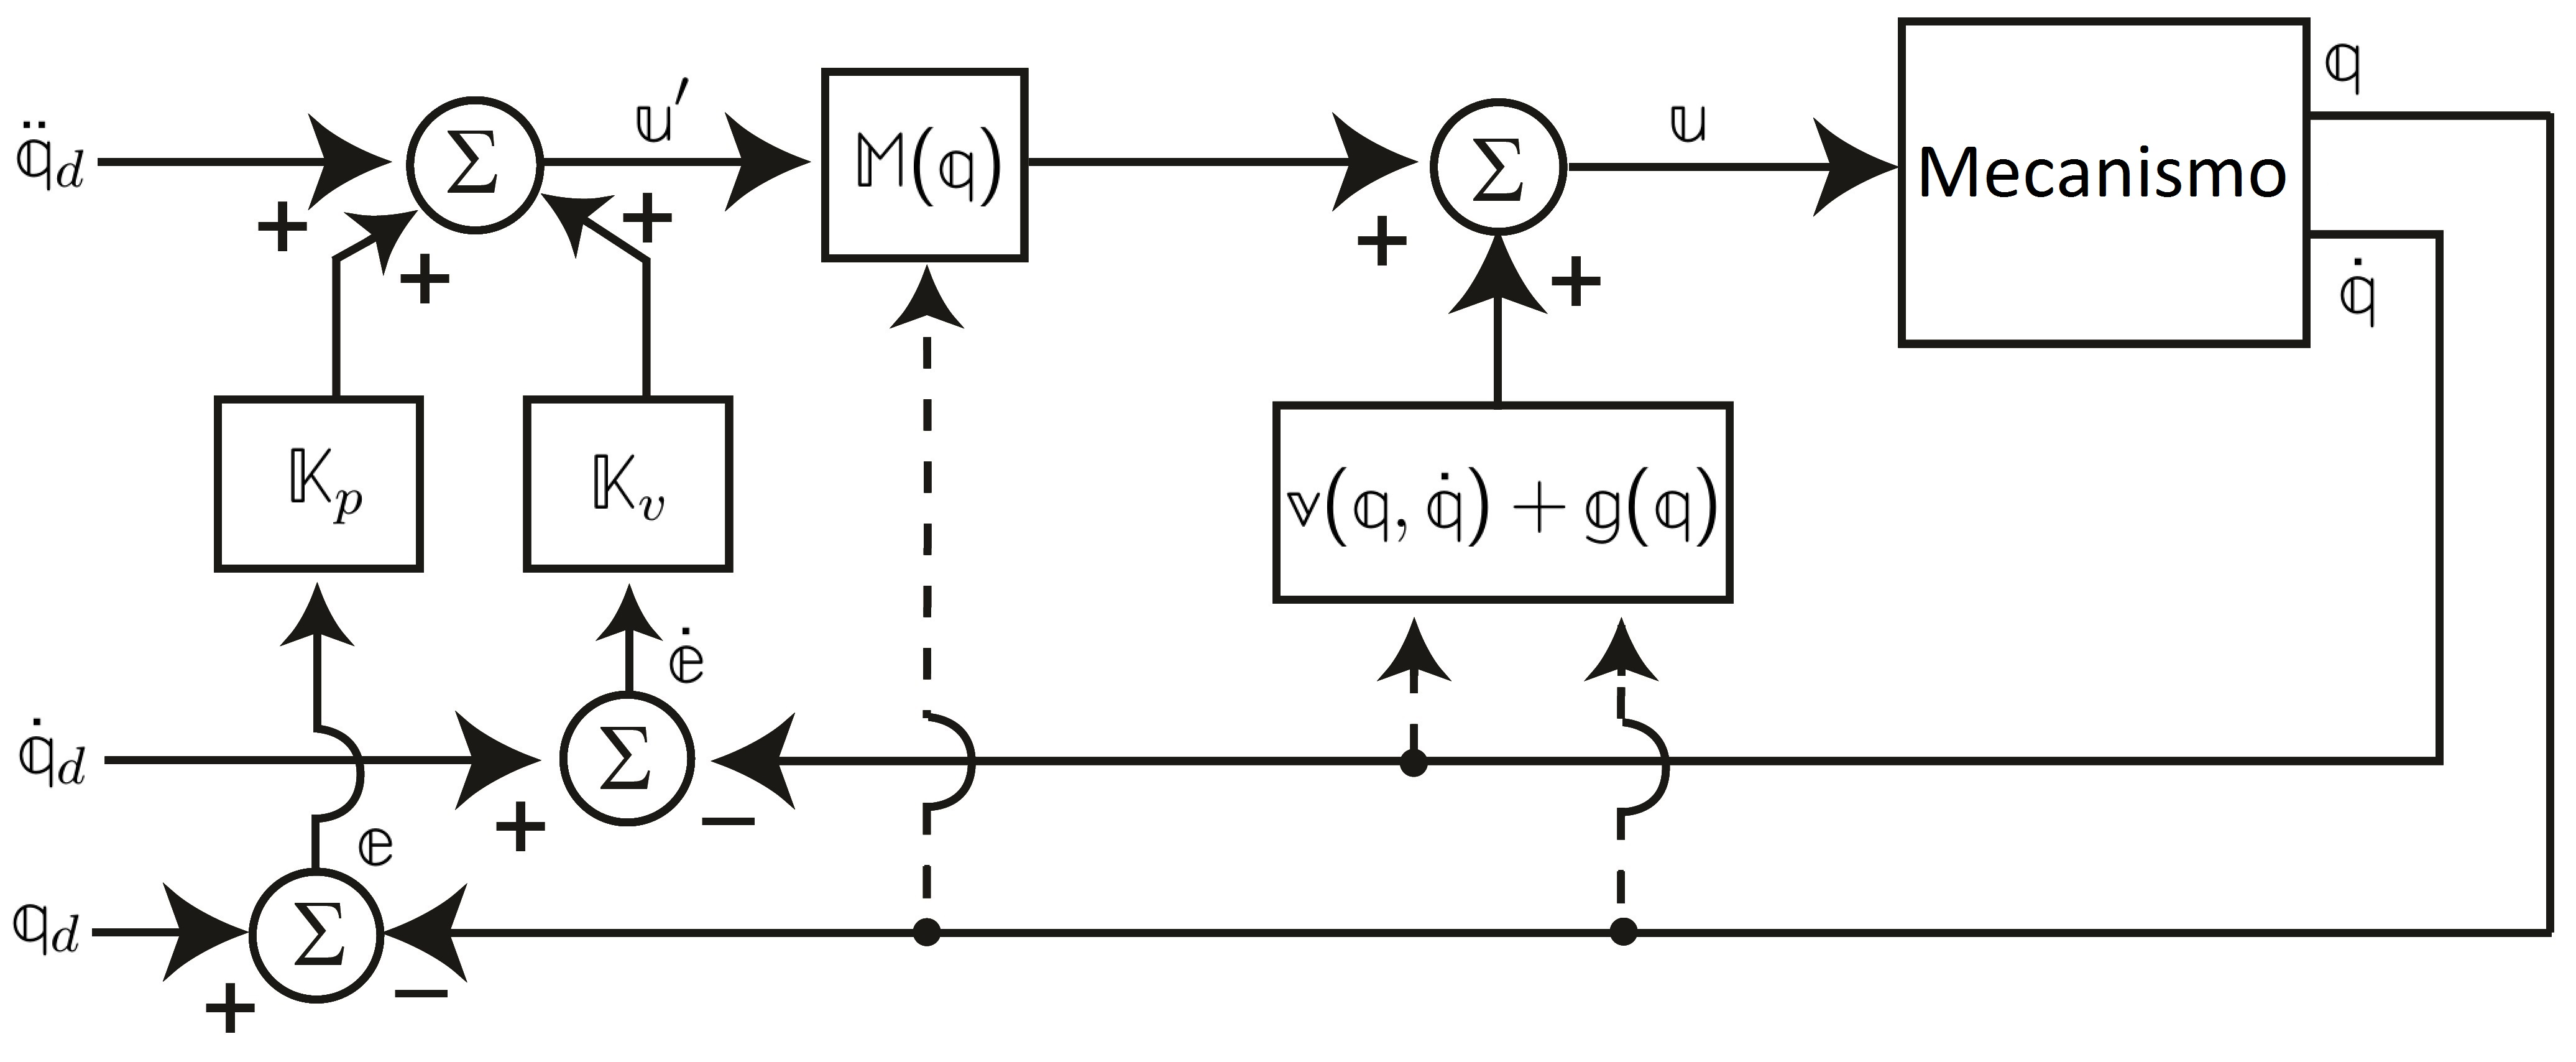
\includegraphics[scale=0.385]{../figures/CTC.jpg}  
	\caption{Malha de CTC (Adaptado de \cite{Craig})}
	\label{fig:CTC}
\end{figure}

Visando a redução do custo computacional associado ao cálculo do modelo dinâmico em tempo real, alguns autores propõe a utilização do CTC com pré-alimentação (CTCp) \cite{Khalil, Siciliano, Spong}. Essa técnica é similar ao CTC, com a diferença de que a compensação das não linearidades é feita por pré-alimentação e não mais por realimentação.  Consequentemente, realiza-se o cálculo do modelo dinâmico previamente, diminuindo o custo computacional.

De fato, Codourey \cite{Codourey} obteve uma redução de 600\% no erro de posição utilizando o CTCp em um ensaio experimental com o robô DELTA, ao substituir os PDs originais. Na simulação do controle de um mecanismo 6-UPS, Wang et al. \cite{Wang} utilizaram em cascata controladores lineares de posição, velocidade e corrente em cada junta ativa, além de  uma compensação dinâmica por pré-alimentação dos distúrbios de torque.

\begin{figure}[h]
	\centering
	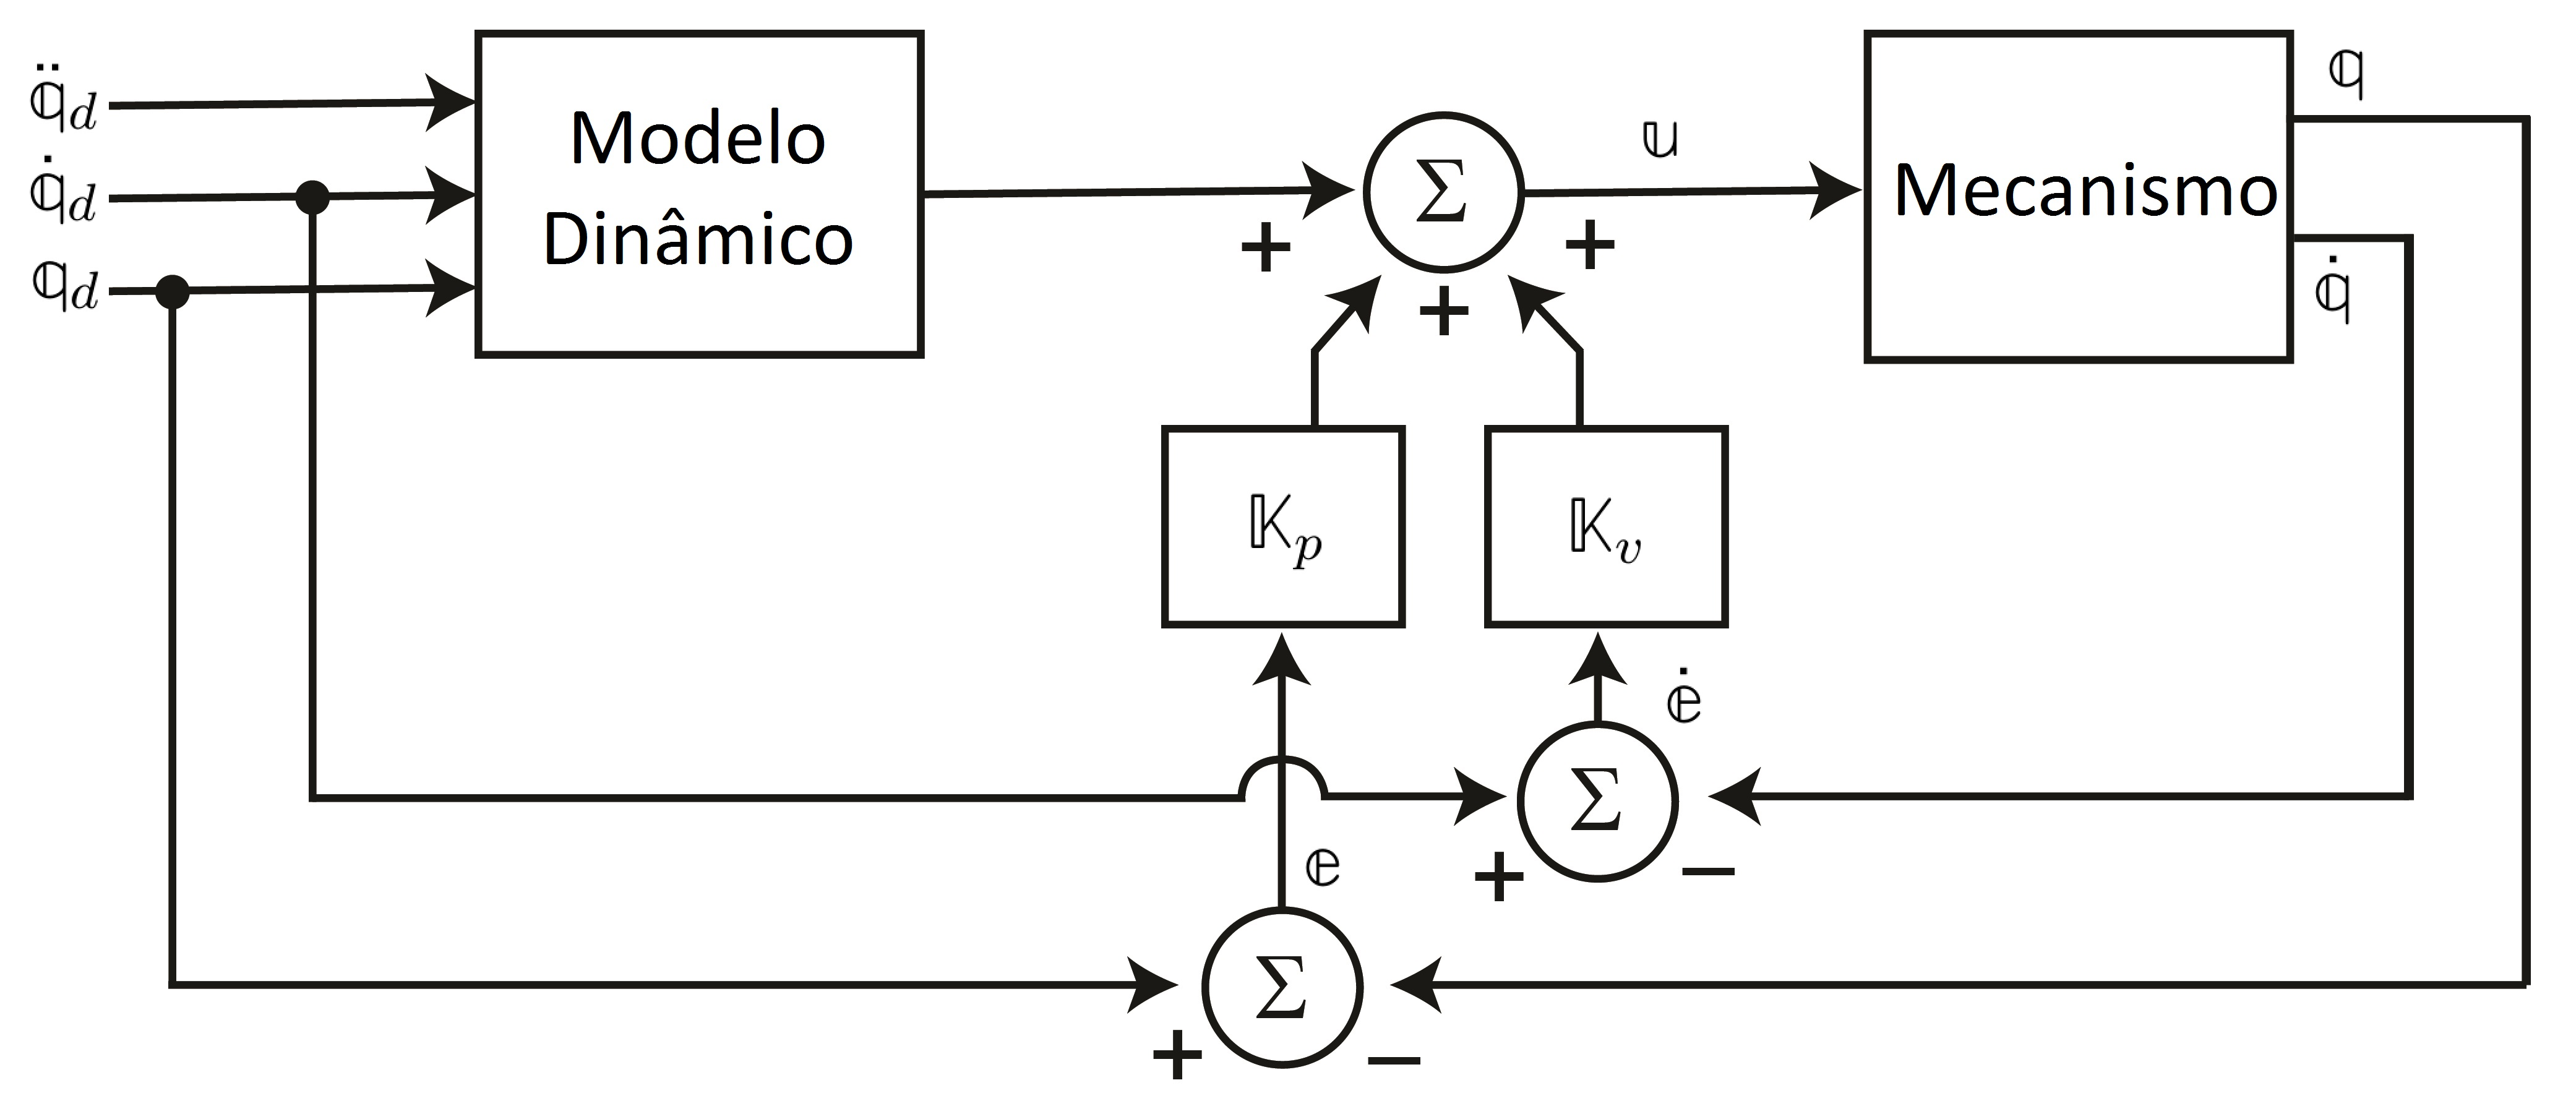
\includegraphics[scale=0.385]{../figures/CTCp.jpg}  
	\caption{Malha de CTCp (Adaptado de \cite{Craig})}
	\label{fig:CTCp}
\end{figure}

Com o intuito de melhorar a robustez do CTC associada a incertezas paramétricas, Zubizarreta et al. \cite{Zubizarreta, Zubizarreta2, Zubizarreta3, Zubizarreta4} propuseram  o  Controle por Torque Computado Estendido (CTCe), que utiliza informação redundante obtida pelo sensoriamento de juntas passivas. Em \cite{Zubizarreta}, os controladores propostos demonstraram maior robustez, principalmente em relação a parâmetros cinemáticos, durante as simulações realizadas com o mecanismo 3-RRR.

Outra técnica alternativa, aplicada a mecanismos paralelos, é o controle preditivo baseado em modelo (CPM). Para a sua implementação, o CPM necessita minimizar uma função objetivo, dependente das saidas e do esforço de controle, ambos calculados em tempo futuro \cite{Camacho}. Assim, dependendo do modelo utilizado, o processo de otimização pode agregar um custo computacional que inviabilize o controle, comprometendo a motivação inicial de aprimorar o desempenho do sistema. Como exemplos de utilização do CPM, podem ser citados os trabalhos de Vivas et al. \cite{Vivas} e   Duchaine et al. \cite{Duchaine}.

Com o propósito de controlar o mecanismo H4, Vivas et al. \cite{Vivas} utilizaram  uma malha de CPM linear e outra malha para compensação das não linearidades. Após a comparação do desempenho do controlador proposto com  o CTC, os autores observaram maior robustez do CPM a incertezas paramétricas. 

Duchaine et al. \cite{Duchaine}, por sua vez, propuseram um controlador preditivo baseado no modelo não linear de um mecanismo paralelo de 6 graus de liberdade. Visando a obtenção de uma solução analítica para o problema de otimização, foram adotadas diversas hipóteses simplificadoras no modelo dinâmico do mecanismo. Com o intuito de comparar o controlador proposto com um PID, foram feitos alguns experimentos, onde se observou  que o CPM apresentou erro nulo de posição no final da trajetória, enquanto que o PID demorou um tempo considerável para alcançar erro nulo. Foi verificada a equivalência entre o custo computacional dos 2 controladores. 

O controle adaptativo, também encontrado na literatura, caracteriza-se pela utilização de leis de adaptação para realizar a estimação em tempo real de parâmetros do sistema ou de termos de compensação dinâmica. Sendo assim, as técnicas de controle adaptativo possibilitam que o sistema se torne praticamente insensível a incertezas paramétricas. Para o caso em que se realiza a estimação em tempo real dos parâmetros do sistema, pode-se dizer que o custo computacional é superior ao do CTC, visto que é necessário integrar as leis de adaptação em tempo real. Além disso, é necessário obter o modelo dinâmico linear em relação aos parâmetros do sistema \cite{SlotiniA}, o que pode ser uma tarefa difícil, inviabilizando, em alguns casos, a aplicação da técnica. Em \cite{Codourey2} é proposto um algoritmo de obtenção do modelo dinâmico simplificado de mecanismos paralelos nesse formato.

Em \cite{SlotiniA} é proposta uma lei de controle que combina o controle adaptativo com a técnica de controle robusto conhecida por Controle por Modos Deslizantes. Chemori et al. \cite{Chemori} utilizaram essa técnica  com o intuito de diminuir os erros de posição em regime permanente no controle de um mecanismo paralelo do tipo PAR2. Por outro lado, Honegger at al. \cite{Honegger} empregaram o controle adaptativo com estimação em tempo real dos parâmetros do sistemas, realizando a compensação dinâmica por pré-alimentação, em um mecanismo  paralelo do tipo Hexaglide.

\begin{figure}[h]
	\centering
	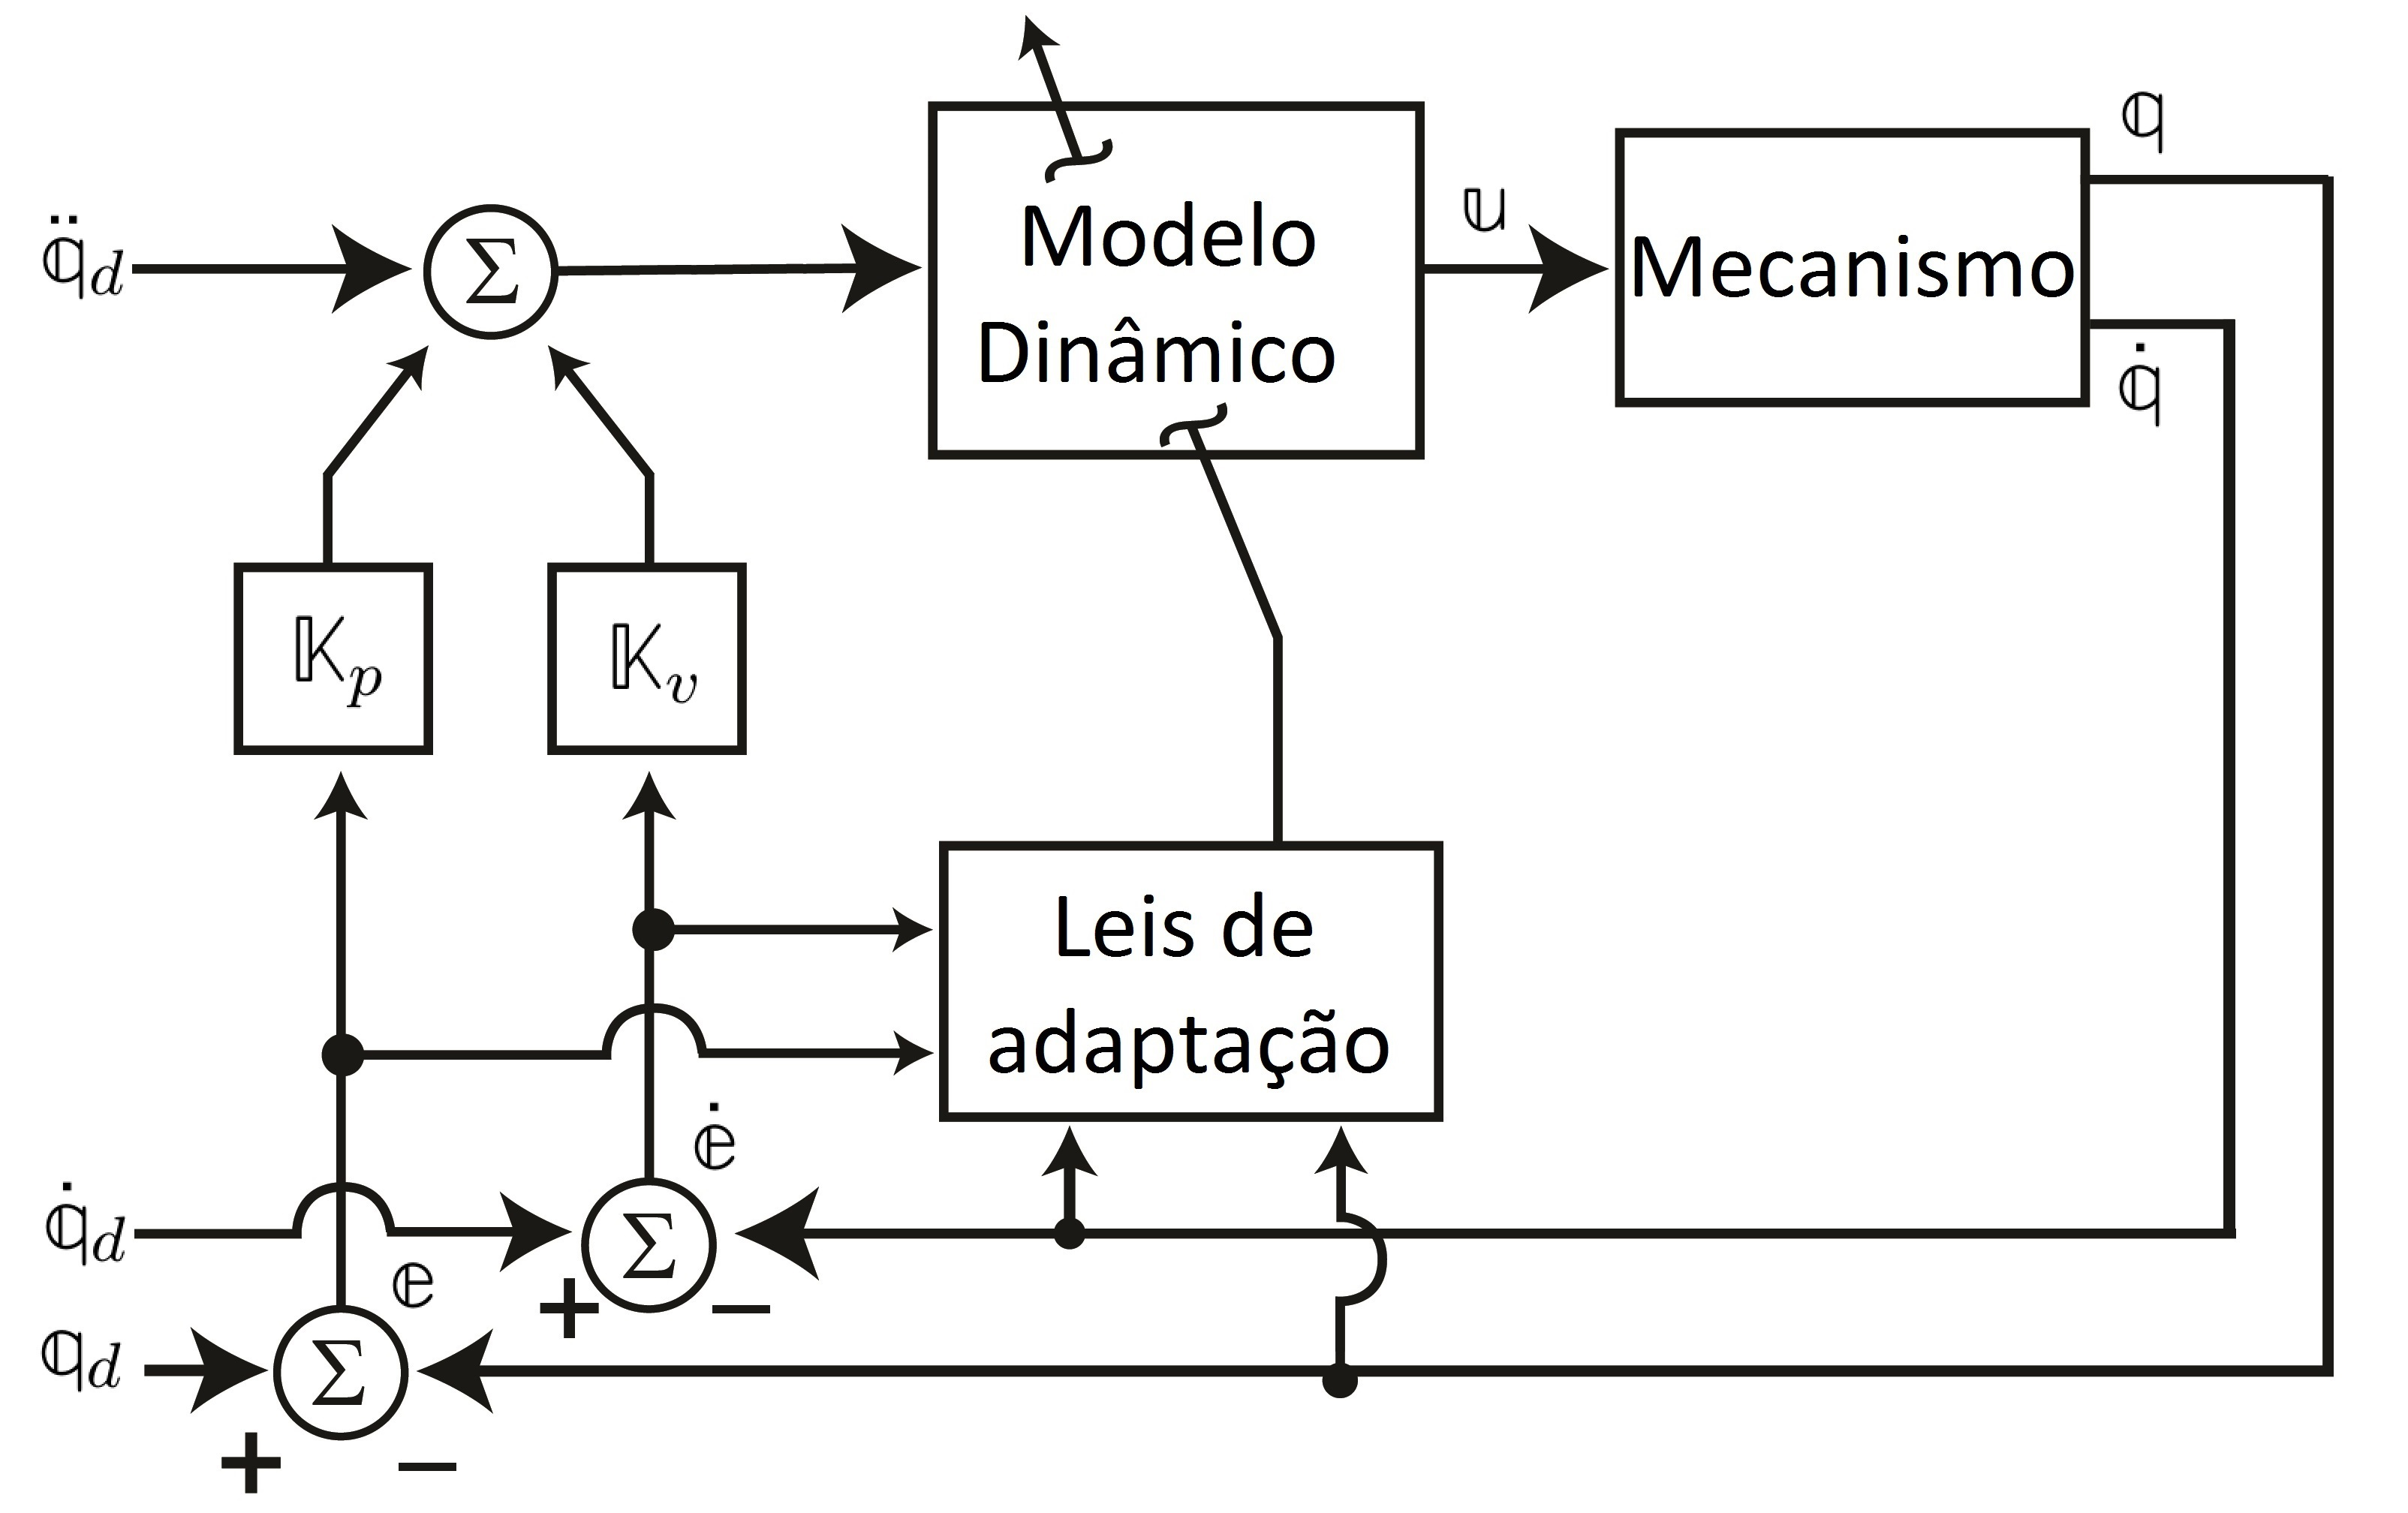
\includegraphics[scale=0.385]{../figures/CA.jpg}  
	\caption{Malha de controle adaptativo (Adaptado de \cite{Craig})}
	\label{fig:CTCp}
\end{figure}

Outra técnica promissora para aplicação em mecanismos paralelos é o Controle por Modos Deslizantes (CMD). A técnica consiste no projeto de leis de controle que levem o sistema para superfícies de escorregamento no espaço de fase, de modo que assim que o sistema atinje e é mantido nas superfícies de escorregamento, o erro de controle decai exponencialmente para zero \cite{Slotini}. Para garantir que o sistema atinja em tempo finito e se mantenha nas superfícies de escorregamento, são utilizados termos descontínuos na lei de controle, o que pode causar problemas de oscilações bruscas em alta frequência nos esforços de controle ({\em chattering}). Em \cite{Guldner}  e  \cite{Utkin2} são propostas técnicas para evitar esse tipo de problema. A grande vantagem da utilização deste tipo de lei de controle é sua grande robustez a incertezas estruturadas e não estruturadas, sendo possível realizar o projeto do controlador de modo a suprimir um dado nível de incertezas paramétricas. Em \cite{SlotiniSMC} é proposta uma metodologia de projeto de Controle por Modos Deslizantes para manipuladores robóticos seriais.

Na literatura são encontradas diversos artigos utilizando a técnica de CMD aliada à lógica {\em fuzzy} e/ou redes neurais para o controle de manipuladores robóticos \cite{Begon, Ertugrul, Hu, Sadati}. Begon et al. \cite{Begon} propuseram uma lei de controle baseada na teoria de CMD e na utilização de lógica {\em fuzzy} para controlar de maneira independente os atuadores de um mecanismo paralelo do tipo Hexa. A técnica proposta teve o intuito de obter a robustez característica do CDM sem necessitar de uma lei de controle com termos descontínuos, evitando o {\em chattering}.

Em \cite{Zeinali}, Zeinali et al. desenvolveram uma lei de controle  baseada nas teorias de CMD e controle adaptativo. O controlador desenvolvido realiza a compensação dinâmica em tempo real do erro de modelagem através de uma lei de adaptação. Além disso, substitui o termo descontínuo da lei de controle por um termo do tipo PID, com o intuito de evitar o {\em chattering}. A estabilidade e robustez da lei de controle proposta foram provadas utilizando a teoria de estabilidade de Lyapunov \cite{Slotini}. A robustez da lei de controle foi verificada através de simulações do controlador proposto aplicado a um mecanismo serial do tipo \underline{R}\underline{R}, nas quais o controlador conseguiu manter erros de posição muito pequenos em regime permanente, mesmo sendo baseado em um modelo muito pobre e na presença de distúrbios de torque. A técnica apresentada se mostra promissora, porém, como no artigo foi feita apenas a simulação da lei de controle em um mecanismo serial bidimensional, ainda não se pode afirmar nada sobre seu desempenho em mecanismos paralelos tridimensionais.

\section{Bancada de ensaios}

%METODOLOGIA--------------------------------------------------------------------
\chapter{Metodologia da Pesquisa}\label{method}

Fundamentalmente, a metodologia desta pesquisa compreende a execução de seis fases, abrangendo desde o desenvolvimento de algoritmos para as modelagens cinemática e dinâmica ao projeto de controladores e sua validação experimental.

\section{Primeira fase} 
Desenvolver um algoritmo genérico, capaz de gerar os modelos dinâmicos completos de mecanismos paralelos que operem em espaço plano, esférico ou tridimensional. Esta geração parte da definição da topologia do mecanismo paralelo, suas cadeias cinemáticas, descrevendo a localização relativa de seus elos e juntas. 

Dentre os efeitos de modelagem considerados, destacam-se os decorrentes da inércia efetiva e acoplada, das forças de Coriolis e centrífugas, da força gravitacional, bem como dos esforços dos atuadores. Pretende-se que a geração dos modelos seja realizada de forma implícita. Para tanto, será empregado o método Recursivo Modular de Modelagem (RMM) proposto por Orsino [36] que, por meio da definição de níveis hierárquicos da estrutura de um sistema mecânico e a descrição da dependência das variáveis cinemáticas envolvidas,  permite o acoplamento de subsistemas multicorpos.

\section{Segunda fase} 
Efetuar as modelagens cinemática e dinâmica do mecanismo articulado plano 5R [34], utilizando o algoritmo desenvolvido na fase anterior.

\section{Terceira fase} 
Nesta fase, diferentes técnicas de controle serão avaliadas sob a perspectiva de sua utilização em manipuladores paralelos. Assim, 
em princípio, esta pesquisa foca na síntese de um controlador não-linear robusto e de alto desempenho. Para tanto, serão consideradas as incertezas paramétricas e a possibilidade de atuação redundante [11], além de estratégias para a determinação de leis de controle com custo computacional
consideralvemente menor do que as tradicionais, que empreguem o Controle por Torque Computado [15, 55].

\section{Quarta fase} Avaliar o emprego de diferentes técnicas de controle de trajetória aplicadas especificamente para o manipulador 5R,
empregando a metodologia da terceira fase.

\section{Quinta fase} Realizar diversas simulações que permitam observar a consistência dos resultados, no tocante às análises cinemáticas direta e inversa, bem como das análises dinâmicas direta e inversa. Além disso, serão determinadas as respostas dinâmicas do manipulador sujeito às distintas leis de controle sintetizadas.

\section{Sexta fase} 
De modo a avaliar o desempenho previsto pelo uso de diferentes controladores para o manipulador paralelo 5R, será realizada a validação experimental em uma das bancadas de ensaio do LaMMaR. Para tanto, serão escolhidas duas trajetórias: uma que considere o comportamento em regime permanente e outra em regime transitório. 

Neste sentido, almeja-se observar se haverá alguma diferença de desempenho se o controle for executado no espaço das juntas ou no da tarefa. Além disso, pretende-se considerar os efeitos da implementação de técnicas de controle puras ou combinadas.
Para auxiliar na comparação entre as técnicas de controle, serão definidas duas métricas: uma que considere o erro de posicionamento do efetuador e outra a magnitude dos torques dos atuadores.

\section{O que tinha antes} 
O estágio atual de desenvolvimento do presente projeto ocorre basicamente em três áreas:
aplicação do algoritmo de modelagem e simulação para os mecanismos 5R \cite{22orsino} e 2\underline{R}SU + \underline{P}PaP \cite{Kumazawa}, o projeto e simulação de controladores não lineares robustos de alto desempenho baseado no modelo dinâmico para os mecanismos citados, e a validação experimental das leis de controle sintetizadas.

Os trabalhos no âmbito de modelagem e simulação estão sendo desenvolvidos a partir da aplicação do algoritmo de modelagem cinemática e dinâmica de mecanismos paralelos desenvolvido, baseado na utilização dos parâmetros de Denavit-Hartenberg \cite{Craig, Denavit, Lipkin} e no método Orsino de acoplamento de subsistemas \cite{23orsino}. Toda modelagem será feita em C++, utilizando uma biblioteca otimizada de cálculo matricial (Armadillo).
As simulações da dinâmica direta do mecanismo serão feitas utilizando o método Runge-Kutta de 8ª ordem \cite{RK} para solução de sistemas de EDOs, de modo a garantir estabilidade numérica do método, mesmo utilizando leis de controle quase descontínuas.

Os trabalhos na área de projeto de controle serão feitos utilizando a metodologia desenvolvida de projeto de controladores robustos multivariáveis para mecanismos paralelos, baseada no modelo dinâmico do mecanismo a ser controlado e na técnica de controle por modos deslizantes \cite{Slotini, Utkin}.

Os trabalhos no âmbito da validação experimental das leis de controle sintetizadas serão realizados no protótipo do mecanismo 5R que encontra-se no laboratório de mecanismos. A bancada experimental do mecanismo 5R já está funcional e já forem realizados alguns testes de leis de controle de trajetória baseadas no modelo dinâmico do mecanismo. Para a realização da validação experimental nesta bancada, será realizada a identificação dos parâmetros do sistema e suas respectivas incertezas, projeto do controlador baseado nos parâmetros e incertezas identificadas, implementação das leis de controle, e aquisição de dados. \\

\begin{figure}[h!]
	\centering
	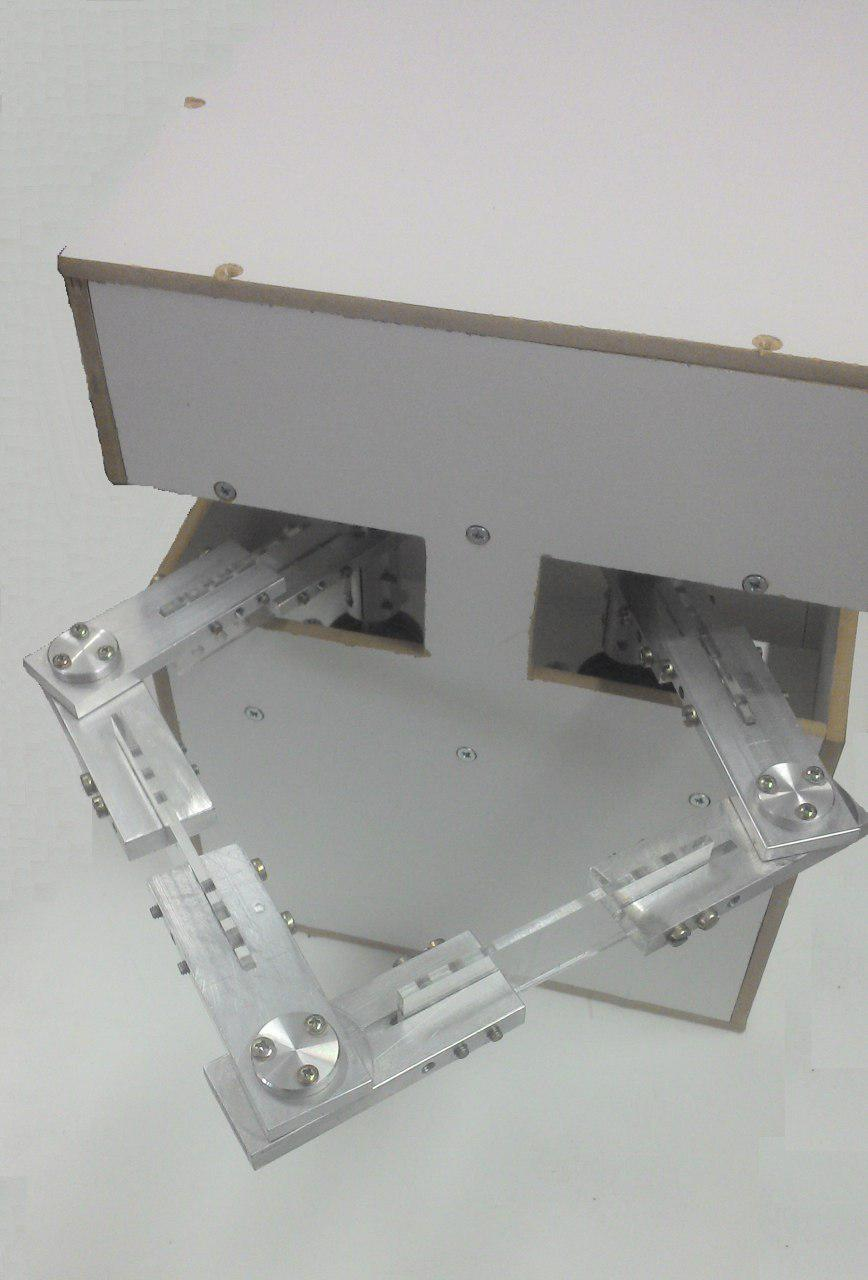
\includegraphics[scale=0.3]{../figures/Clara.jpg}  
	\caption{Protótipo do mecanismo 5R}
	\label{fig:Mecanismo2}
\end{figure}

%MODELAGEM DE MANIPULADORES SERIAIS--------------------------------------------

\part{Modelagem}
	
\chapter{Modelagem de manipuladores seriais}
\capepigrafe[0.5\textwidth]{``Frase espirituosa de um autor famoso''}{Autor famoso}

Este capítulo tem o intuito de apresentar um algoritmo genérico para a obtenção do modelo cinemático e dinâmico de mecanismos seriais. O algoritmo apresentado é implementável em linguagens de programação comumente usadas atualmente, como C++, Java e Python, sem necessitar de recursos de manipulação simbólica. \\
Para a obtenção do modelo, são necessários apenas os parametros de Denavit-Hartemberg \cite{Craig, Denavit, Lipkin, Cabral} do mecanismo e as posições dos centros de massa dos ligamentos em relação aos sistemas de coordenadas fixos aos ligamentos. \\ 

Seja $\ssB$ um sistema mecânico serial de $\nu$ graus de liberdade. Primeiramente, fazemos as seguintes definições:

\begin{itemize}
\item $\llN$ ou $\llB_0$: referencial inercial.
\item $\ttN$ ou $\ttB_0$: sistema de coordenadas da base do mecanismo, fixo a $\llN$.
\item $\llB_i, \,i=1,...,\nu$: i-ésimo ligamento.
\item $\ttB_i, \,i=1,...,\nu$: sistema de coordenadas solid\'ario a $\llB_i$.
\item $\tto_i, \,i=0,...,\nu$: origem do sistema $\ttB_i$.
\item $\{\vi_i, \vj_i, \vk_i\}, \,i=0,...,\nu$: base ortonormal do sistema $\ttB_i$.
\item $\ttg_i, \,i=1,...,\nu$: centro de massa de $\llB_i$.
\item $\ttx$: ponto no espa\c{c}o fixo ao efetuador.
\item $m_i$: massa da barra $\llB_i$.
\item $\vI_{\ttg_i}$: tensor de in\'ercia da barra $\llB_i$ em relação a seu centro de massa.
\item $\mI_i$: tensor de in\'ercia $\vI_{\ttg_i}$ escrito na base $\ttN$, ou seja, $\vct{\vI_{\ttg_i}}_{\ttN \rl \ttN}$.
\item $q_i, \,i=1,...,\nu$: deslocamento relativo (angular ou linear) da i-ésima junta.
\item  $\mq$: matriz-coluna de $\nu$ coordenadas generalizadas independentes. É dada por $\mq = \begin{bmatrix}
q_1 & ... & {q}_{\nu}
\end{bmatrix}^\msT $.
\item $\vg$: Vetor aceleração gravitacional.
\item $\mgamma$: Vetor aceleração gravitacional escrito na base $\ttN$, ou seja, $\vct{\vg}_{\ttN}$.
\item $\vf_i$: Vetor força não-reativa resultante aplicada no centro de massa de $\llB_i$.
\item $\vtau_i$: Vetor torque não-reativo resultante aplicado em $\llB_i$.
\item $\overline{\mf}_i$: Matriz-coluna de forças não-reativas generalizadas aplicadas no subsistema $\llB_i$. É dada por $\overline{\mf}_i = \begin{bmatrix}
\vct{\vf_i}_\ttN^\msT &
\vct{\vtau_i}_\ttN^\msT
\end{bmatrix}^\msT $.
\end{itemize}

\section{Cinemática}

\subsection{Cinemática de posição}\label{S05-02-01-01}

Dados os parâmetros de Denavit-Hartemberg $a_i$, $\alpha_i$, $d_i$ e $\theta_i$, com $1 \leq i \leq \nu$, é possível obter as matrizes de transformação homogênea $\hvct{\vone}_{\ttB_{i-1} \rl \ttB_i}$ a partir da seguinte expressão \cite{Cabral} :

\begin{empheq}[box=\myyellowbox]{equation} \label{eq:TransformacaoHomogeneaDH}
\hvct{\vone}_{\ttB_{i-1} \rl \ttB_i} =
\begin{bmatrix}
\ccos\theta_i & -\ssin\theta_i \ccos\alpha_i &  \ssin\theta_i \ssin\alpha_i & a_i\ccos\theta_i \\
\ssin\theta_i &  \ccos\theta_i \ccos\alpha_i & -\ccos\theta_i \ssin\alpha_i & a_i\ssin\theta_i \\
0             &  \ssin\alpha_i               &  \ccos\alpha_i               & d_i \\
0             & 0                            & 0                            & 1
\end{bmatrix},\, i=1,...,\nu
\end{empheq}

Tendo obtido $\hvct{\vone}_{\ttB_{i-1} \rl \ttB_i}$, é possível obter as transformações homogêneas que relacionam os sistemas solidários aos ligamentos ($\ttB_i$) ao sistema da base ($\ttN$) pela seguinte expressão recursiva:

\begin{empheq}[box=\myyellowbox]{equation} \label{eq:H__}
\hvct{\vone}_{\ttN \rl \ttB_i} =
\begin{cases}
\hvct{\vone}_{\ttB_0 \rl \ttB_1}, \text{se } i=1 \\
\hvct{\vone}_{\ttN \rl \ttB_{i-1}} \cdot \hvct{\vone}_{\ttB_{i-1} \rl \ttB_i}  , \text{se } i>1
\end{cases} \, i=1,...,\nu
\end{empheq}

As matrizes  $\hvct{\vone}_{\ttN \rl \ttB_i}$ apresentam o seguinte formato:
\begin{empheq}[box=\lightbluebox]{equation} \label{eq:H__2}
\hvct{\vone}_{\ttN \rl \ttB_i} =
\begin{bmatrix}
\vct{\vi_{i}}_{\ttN} & \vct{\vj_{i}}_{\ttN} & \vct{\vk_{i}}_{\ttN} & \vct{\tto_i}_{\ttN} \\
0 & 0 & 0 & 1
\end{bmatrix}
\end{empheq}

Sendo assim, tendo obtido $\hvct{\vone}_{\ttN \rl \ttB_i}$, automaticamente obtemos $\vct{\vi_{i}}_{\ttN}, \vct{\vj_{i}}_{\ttN}, \vct{\vk_{i}}_{\ttN}$ e $\vct{\tto_i}_{\ttN}$. Note que também obtemos as coordenadas do efetuador no sistema da base, pois
\begin{empheq}[box=\myyellowbox]{equation} \label{eq:x_}
\vct{\ttx}_{\ttN} = \vct{\tto_{\nu}}_{\ttN}
\end{empheq}

Além disso, como $\vct{\ttg_i}_{\ttB_i}$ são dados de entrada do algoritmo, obtemos as coordenadas dos centros de massa dos ligamentos no sistema da base através da seguinte expressão:
\begin{empheq}[box=\myyellowbox]{equation} \label{eq:og__}
\hvct{\ttg_i}_{\ttN} = \hvct{\vone}_{\ttN \rl \ttB_i} \cdot \hvct{\ttg_i}_{\ttB_i}
\end{empheq}

\subsection{Cinemática de velocidades lineares}\label{S05-02-01-02}

A velocidade do efetuador pode ser obtida aplicando recursivamente o príncipio da composição de movimentos para velocidades lineres deduzido anteriormente \eqref{eq:Composicao_vel}:

\begin{equation}
\vv_{\ttx}^{\lllB_0} = \vv_{\ttx \rl \lllB_1}^{\lllB_0} + \vv_{\ttx}^{\lllB_1}
\end{equation}
\begin{equation}
\vv_{\ttx}^{\lllB_1} = \vv_{\ttx \rl \lllB_2}^{\lllB_1} + \vv_{\ttx}^{\lllB_2}
\end{equation}
$$ \vdots $$
\begin{equation}
\vv_{\ttx}^{\lllB_{i-1}} = \vv_{\ttx \rl \lllB_i}^{\lllB_{i-1}} + \vv_{\ttx}^{\lllB_i}
\end{equation}
$$ \vdots $$
\begin{equation}
\vv_{\ttx}^{\lllB_{\nu-1}} = \vv_{\ttx \rl \lllB_\nu}^{\lllB_{\nu-1}} + \vv_{\ttx}^{\lllB_\nu}
\end{equation}

Como $\ttx$ é fixo a $\llB_\nu$, temos que:
\begin{equation}
\vv_{\ttx}^{\lllB_\nu} = \vzr
\end{equation}

Sendo assim, a velocidade do efetuador em relação a cada um dos referenciais pode ser obtida recursivamente pela seguinte expressão:
%\begin{equation}
%\vv_{\ttx}^{\lllB_{i-1}} =
%\begin{cases}
%\displaystyle\sum_{j=i}^{\nu} \vv_{\ttx \rl \lllB_{j}}^{\lllB_{j-1}}, \; 1 \leq i \leq \nu \\
%\vzr, \;\;\;\;\;\;\;\;\;\;\;\; i = \nu + 1
%\end{cases}\, i=1,...,\nu+1
%\end{equation}
\begin{equation}
\vv_{\ttx}^{\lllB_{i-1}} =
\begin{cases}
\vzr, \;\;\;\;\;\;\;\;\;\;\;\;\;\;\; i = \nu + 1 \\
\vv_{\ttx}^{\lllB_{i}} + \vv_{\ttx \rl \lllB_{i}}^{\lllB_{i-1}}, \; 1 \leq i \leq \nu \\
\end{cases}\, i=\nu+1,...,1
\end{equation}



Sendo que, a partir da equação \eqref{eq:Poisson_v}, a velocidade de arrastamento de cada uma das juntas é dada por:
\begin{equation}
\vv_{\ttx \rl \lllB_{i}}^{\lllB_{i-1}} = 
\begin{cases}
\dot{q}_{i} \vk_{i-1}, \;\;\;\;\;\;\;\;\;\;\;\;\;\; \text{i-ésima junta prismática} \\
\dot{q}_{i} \vk_{i-1} \wedge \vr_{\tto_{i-1} \rl \ttx}, \; \text{i-ésima junta rotativa}
\end{cases}\, i=1,...,\nu
\end{equation}

Fazendo as seguintes definições:
\begin{empheq}[box=\myyellowbox]{equation} \label{eq:jvi_}
\mj_{v\,i}(\mq) = \begin{cases}
\vct{\vk_{i-1}}_{\ttN}, \;\;\;\;\;\;\;\;\;\;\;\;\;\;\;\;\;\;\;\;\;\;\;\;\;\;\; \text{i-ésima junta prismática} \\
\vct{\vk_{i-1}}_{\ttN}\wedge (\vct{\ttx}_{\ttN}-\vct{\tto_{i-1}}_{\ttN}) , \; \text{i-ésima junta rotativa} \\
\end{cases} \, i=1,...,\nu
\end{empheq}

\begin{empheq}[box=\lightbluebox]{equation}
\mv_i = \vct{\vv_{\ttx}^{\lllB_{i}} }_{\ttN}
\end{empheq}

\begin{empheq}[box=\lightbluebox]{equation}
\mv^\star  = \mv_0 =\vct{\vv_{\ttx}^{\lllN} }_{\ttN}
\end{empheq}

Temos que:
\begin{equation}
\vct{\vv_{\ttx \rl \lllB_{i}}^{\lllB_{i-1}} }_{\ttN} = \mj_{v\,i} \dot{q}_{i}, \; i=1,...,\nu
\end{equation}
\begin{empheq}[box=\myyellowbox]{equation}
\mv_{i-1} =
\begin{cases}
\mzr, \;\;\;\;\;\;\;\;\;\;\;\;\; i = \nu + 1 \\
\mv_i + \mj_{v\,i}  \dot{q}_{i}, \; 1 \leq i \leq \nu \\
\end{cases}\, i=\nu+1,...,1
\end{empheq}

\begin{empheq}[box=\lightbluebox]{equation}\label{eq:vel_est}
\mv^\star (\mq, \dot{\mq}) = \mJ_v(\mq) \cdot \dot{\mq}
\end{empheq}

Sendo:
\begin{empheq}[box=\myyellowbox]{equation} \label{eq:Jv_}
\mJ_v(\mq) = \begin{bmatrix}
\mj_{v\,1}(\mq) & ... & \mj_{v\,\nu}(\mq)
\end{bmatrix}
\end{empheq}

Para obter as velocidades dos centros de massa dos ligamentos, seguimos a mesma linha de raciocínio e obtemos os seguintes resultados:

Definindo:
\begin{empheq}[box=\myyellowbox]{equation} \label{eq:jvij_}
\mj_{v\,i,j}(\mq) = \begin{cases}
\mzr, \;\;\;\;\;\;\;\;\;\;\;\;\;\;\;\;\;\;\;\;\;\;\;\;\;\;\;\;\;\;\;\;\;\;\;\;\; j>i \\
\vct{\vk_{j-1}}_{\ttN}, \;\;\;\;\;\;\;\;\;\;\;\;\;\;\;\;\;\;\;\;\;\;\;\;\;\;\;\; j\leq i  \text{ e j-ésima junta prismática} \\
\vct{\vk_{j-1}}_{\ttN}\wedge (\vct{\ttg_i}_{\ttN}-\vct{\tto_{j-1}}_{\ttN}) , \; j\leq i \text{ e j-ésima junta rotativa} \\
\end{cases} \, i,j=1,...,\nu
\end{empheq}

\begin{empheq}[box=\lightbluebox]{equation}
\mv_{i,j} = \vct{\vv_{\ttg_i}^{\lllB_{j}}}_{\ttN}
\end{empheq}

\begin{empheq}[box=\lightbluebox]{equation}
\mv^\star_i  = \mv_{i,0} = \vct{\vv_{\ttg_i}^{\lllN} }_{\ttN}
\end{empheq}

Temos:
\begin{empheq}[box=\myyellowbox]{equation} 
\mv_{i,j-1} =
\begin{cases}
\mzr, \;\;\;\;\;\;\;\;\;\;\;\;\;\;\;\;\; j = i+1 \\
\mv_{i,j} + \mj_{v\,i,j} \dot{q}_{j}, \; 1 \leq j \leq i \\
\end{cases}\, i=1,...,\nu, \, j=i+1,...,1
\end{empheq}

\begin{empheq}[box=\lightbluebox]{equation}  \label{eq:v_star_i}
\mv^\star_i(\mq, \dot{\mq}) = \mJ_{v\,i}(\mq) \cdot \dot{\mq}
\end{empheq}

Sendo:
\begin{empheq}[box=\myyellowbox]{equation} \label{eq:Jvi_}
\mJ_{v\,i}(\mq) = \begin{bmatrix}
\mj_{v\,i,1}(\mq) & ... & \mj_{v\,i,\nu}(\mq)
\end{bmatrix}
\end{empheq}

\subsection{Cinemática de velocidades angulares}\label{S05-02-01-03}

A velocidade angular do efetuador pode ser obtida aplicando recursivamente o príncipio da composição de movimentos para velocidades angulares deduzido anteriormente \eqref{eq:composicao_w}:

\begin{equation}
\vomega_{\lllB_\nu}^{\lllB_0} = \vomega_{\lllB_1}^{\lllB_0} + \vomega_{\lllB_\nu}^{\lllB_1}
\end{equation}
\begin{equation}
\vomega_{\lllB_\nu}^{\lllB_1} = \vomega_{\lllB_2}^{\lllB_1} + \vomega_{\lllB_\nu}^{\lllB_2}
\end{equation}
$$ \vdots $$
\begin{equation}
\vomega_{\lllB_\nu}^{\lllB_{i-1}} = \vomega_{\lllB_i}^{\lllB_{i-1}} + \vomega_{\lllB_\nu}^{\lllB_i}
\end{equation}
$$ \vdots $$
\begin{equation}
\vomega_{\lllB_\nu}^{\lllB_{\nu-2}} = \vomega_{\lllB_{\nu-1}}^{\lllB_{\nu-2}} + \vomega_{\lllB_\nu}^{\lllB_{\nu-1}}
\end{equation}


Sendo assim, a velocidade angular do efetuador em relação a cada um dos referenciais pode ser obtida recursivamente pela seguinte expressão:
%\begin{equation}
%\vomega_{\lllB_\nu}^{\lllB_{i-1}} =
%\begin{cases}
%\displaystyle\sum_{j=i}^{\nu} \vomega_{\lllB_{j}}^{\lllB_{j-1}}, \; 1 \leq i \leq \nu \\
%\vzr, \;\;\;\;\;\;\;\;\;\;\;\; i = \nu + 1
%\end{cases}\, i=1,...,\nu+1
%\end{equation}
\begin{equation}
\vomega_{\lllB_\nu}^{\lllB_{i-1}} =
\begin{cases}
\vzr, \;\;\;\;\;\;\;\;\;\;\;\;\;\;\;\; i = \nu + 1 \\
\vomega_{\lllB_\nu}^{\lllB_{i}} + \vomega_{\lllB_{i}}^{\lllB_{i-1}}, \; 1 \leq i \leq \nu \\
\end{cases}\, i=\nu+1,...,1
\end{equation}



Sendo que a velocidade angular de arrastamento de cada uma das juntas é dada por:
\begin{equation}
\vomega_{\lllB_{i}}^{\lllB_{i-1}} = 
\begin{cases}
\vzr, \;\;\;\;\;\;\; \text{i-ésima junta prismática} \\
\dot{q}_{i} \vk_{i-1}, \; \text{i-ésima junta rotativa}
\end{cases}\, i=1,...,\nu
\end{equation}

Fazendo as seguintes definições:
\begin{empheq}[box=\myyellowbox]{equation}  \label{eq:jwi_}
\mj_{\omega\,i}(\mq) = \begin{cases}
\mzr, \;\;\;\;\;\;\;\; \text{i-ésima junta prismática} \\
\vct{\vk_{i-1}}_{\ttN} , \text{i-ésima junta rotativa} \\
\end{cases} \, i=1,...,\nu
\end{empheq}

\begin{empheq}[box=\lightbluebox]{equation}
\momega_i = \vct{\vomega_{\lllB_\nu}^{\lllB_{i}} }_{\ttN}
\end{empheq}

\begin{empheq}[box=\lightbluebox]{equation}
\momega^\star = \momega_0 = \vct{\vomega_{\lllB_\nu}^{\lllN} }_{\ttN} 
\end{empheq}

Temos que:
\begin{equation}
\vct{\vomega_{\lllB_{i}}^{\lllB_{i-1}} }_{\ttN} = \mj_{\omega\,i} \dot{q}_{i}, \; i=1,...,\nu
\end{equation}

\begin{empheq}[box=\myyellowbox]{equation}
\momega_{i-1} =
\begin{cases}
\mzr, \;\;\;\;\;\;\;\;\;\;\;\;\;\; i = \nu + 1 \\
\momega_i + \mj_{\omega\,i} \dot{q}_{i}, \; 1 \leq i \leq \nu \\
\end{cases}\, i=\nu+1,...,1
\end{empheq}

\begin{empheq}[box=\lightbluebox]{equation} \label{eq:vel_ang_est}
\momega^\star(\mq, \dot{\mq}) = \mJ_\omega (\mq) \cdot \dot{\mq}
\end{empheq}

Sendo:
\begin{empheq}[box=\myyellowbox]{equation} \label{eq:Jw_}
\mJ_\omega(\mq) = \begin{bmatrix}
\mj_{\omega\,1}(\mq) & ... & \mj_{\omega\,\nu}(\mq)
\end{bmatrix}
\end{empheq}

Para obter as velocidades angulares de cada ligamentos, seguimos a mesma linha de raciocínio e obtemos os seguintes resultados:

Definindo:
\begin{empheq}[box=\myyellowbox]{equation} \label{eq:jwij_}
\mj_{\omega\,i,j}(\mq) = \begin{cases}
\mzr, \;\;\;\;\;\;\;\;\,  j>i \\
\mj_{\omega\,j}(\mq), \;  j\leq i \\
\end{cases} \, i,j=1,...,\nu
\end{empheq}

\begin{empheq}[box=\lightbluebox]{equation}
\momega_{i,j} = \vct{\vomega_{\lllB_i}^{\lllB_{j}}}_{\ttN}
\end{empheq}

\begin{empheq}[box=\lightbluebox]{equation}
\momega^\star_i = \momega_{i,0} = \vct{\vomega_{\lllB_i}^{\lllN} }_{\ttN} 
\end{empheq}

Temos:
\begin{empheq}[box=\myyellowbox]{equation}
\momega_{i,j-1} =
\begin{cases}
\mzr, \;\;\;\;\;\;\;\;\;\;\;\;\;\;\;\;\;\; j = i+1 \\
\momega_{i,j} + \mj_{\omega\,i,j} \dot{q}_{j}, \; 1 \leq j \leq i \\
\end{cases}\, i=1,...,\nu, \, j=i+1,...,1
\end{empheq}

\begin{empheq}[box=\lightbluebox]{equation} \label{eq:omega_star_i}
\momega^\star_i (\mq, \dot{\mq}) = \mJ_{\omega\,i}(\mq) \cdot \dot{\mq}
\end{empheq}

Sendo:

\begin{empheq}[box=\myyellowbox]{equation} \label{eq:Jwi_}
\mJ_{\omega\,i}(\mq) = \begin{bmatrix}
\mj_{\omega\,i,1}(\mq) & ... & \mj_{\omega\,i,\nu}(\mq)
\end{bmatrix}
\end{empheq}

\subsection{Cinemática de acelerações lineares}\label{S05-02-01-04}

A aceleração do efetuador pode ser obtida aplicando recursivamente o príncipio da composição de movimentos para velocidades lineres deduzido anteriormente \eqref{eq:Composicao_ace}:

\begin{equation}
\va_{\ttx}^{\lllB_0} = \va_{\ttx \rl \lllB_1}^{\lllB_0} + \va_{\ttx}^{\lllB_1} + 2 \vomega_{\lllB_1}^{\lllB_0} \wedge \vv_{\ttx}^{\lllB_1}
\end{equation}
\begin{equation}
\va_{\ttx}^{\lllB_1} = \va_{\ttx \rl \lllB_2}^{\lllB_1} + \va_{\ttx}^{\lllB_2} + 2 \vomega_{\lllB_2}^{\lllB_1} \wedge \vv_{\ttx}^{\lllB_2}
\end{equation}
$$ \vdots $$
\begin{equation}
\va_{\ttx}^{\lllB_{i-1}} = \va_{\ttx \rl \lllB_i}^{\lllB_{i-1}} + \va_{\ttx}^{\lllB_i} + 2 \vomega_{\lllB_i}^{\lllB_{i-1}} \wedge \vv_{\ttx}^{\lllB_i}
\end{equation}
$$ \vdots $$
\begin{equation}
\va_{\ttx}^{\lllB_{\nu-1}} = \va_{\ttx \rl \lllB_\nu}^{\lllB_{\nu-1}} + \va_{\ttx}^{\lllB_\nu} + 2 \vomega_{\lllB_\nu}^{\lllB_{\nu-1}} \wedge \vv_{\ttx}^{\lllB_\nu}
\end{equation}

Como $\ttx$ é fixo a $\llB_\nu$, temos que:
\begin{equation}
\va_{\ttx}^{\lllB_\nu} = \vzr
\end{equation}

Sendo assim, a aceleração do efetuador em relação a cada um dos referenciais pode ser obtida recursivamente pela seguinte expressão:
%\begin{equation}
%\vv_{\ttx}^{\lllB_{i-1}} =
%\begin{cases}
%\displaystyle\sum_{j=i}^{\nu} \vv_{\ttx \rl \lllB_{j}}^{\lllB_{j-1}}, \; 1 \leq i \leq \nu \\
%\vzr, \;\;\;\;\;\;\;\;\;\;\;\; i = \nu + 1
%\end{cases}\, i=1,...,\nu+1
%\end{equation}
\begin{equation}
\va_{\ttx}^{\lllB_{i-1}} =
\begin{cases}
\vzr, \;\;\;\;\;\;\;\;\;\;\;\;\;\;\;\;\;\;\;\;\;\;\;\;\;\;\;\;\;\;\;\;\;\;\;\;\; i = \nu + 1 \\
\va_{\ttx}^{\lllB_i} +\va_{\ttx \rl \lllB_i}^{\lllB_{i-1}} + 2 \vomega_{\lllB_i}^{\lllB_{i-1}} \wedge \vv_{\ttx}^{\lllB_i}, \; 1 \leq i \leq \nu \\
\end{cases}\, i=\nu+1,...,1
\end{equation}



Sendo que, a partir da equação \eqref{eq:Poisson_a}, a aceleração de arrastamento de cada uma das juntas é dada por:
\begin{equation}
\va_{\ttx \rl \lllB_{i}}^{\lllB_{i-1}} = 
\begin{cases}
\ddot{q}_{i} \vk_{i-1}, \;\;\;\;\;\;\;\;\;\;\;\;\;\;\;\;\;\;\;\;\;\;\;\;\;\;\;\;\;\;\;\;\;\;\;\;\;\;\;\;\;\;\;\;\;\;\;\;\;\;\; \text{i-ésima junta prismática} \\
\ddot{q}_{i} \vk_{i-1} \wedge \vr_{\tto_{i-1} \rl \ttx} + \dot{q}^2_{i} \vk_{i-1} \wedge \vk_{i-1} \wedge \vr_{\tto_{i-1} \rl \ttx} , \; \text{i-ésima junta rotativa}
\end{cases}\, i=1,...,\nu
\end{equation}

Fazendo as seguintes definições:
\begin{empheq}[box=\lightbluebox]{equation}
\ma_i = \vct{\va_{\ttx}^{\lllB_{i}} }_{\ttN}
\end{empheq}

\begin{empheq}[box=\lightbluebox]{equation}
\ma^\star = \ma_0 =\vct{\va_{\ttx}^{\lllN} }_{\ttN}
\end{empheq}

Temos que:
\begin{equation}
\vct{\va_{\ttx \rl \lllB_{i}}^{\lllB_{i-1}} }_{\ttN} = \ddot{q}_{i} \mj_{v\,i} + \dot{q}^2_{i} \mj_{\omega\,i} \wedge \mj_{v\,i}, \; i=1,...,\nu
\end{equation}

\begin{empheq}[box=\myyellowbox]{equation}
\ma_{i-1} =
\begin{cases}
\mzr, \;\;\;\;\;\;\;\;\;\;\;\;\;\;\;\;\;\;\;\;\;\;\; i = \nu + 1 \\
\ma_i +  \mj_{v\,i} \ddot{q}_{i} + (\underaccent{\sim}{\ma})_i  , \; 1 \leq i \leq \nu \\
\end{cases}\, i=\nu+1,...,1
\end{empheq}

\begin{empheq}[box=\lightbluebox]{equation} \label{eq:ace_est}
\ma^\star (\mq,\dot{\mq},\ddot{\mq}) = \mJ_v (\mq)  \cdot \ddot{\mq} + \underaccent{\sim}{\ma} (\mq,\dot{\mq})
\end{empheq}

Sendo:
\begin{empheq}[box=\myyellowbox]{equation}
(\underaccent{\sim}{\ma})_i = \dot{q}_{i} \mj_{\omega\,i} \wedge ( \dot{q}_{i}  \mj_{v\,i} + 2  \mv_i)
\end{empheq}

\begin{empheq}[box=\myyellowbox]{equation} \label{eq:a_til}
\underaccent{\sim}{\ma} = \sum_{i=1}^\nu (\underaccent{\sim}{\ma})_i
\end{empheq}

Para obter as acelerações dos centros de massa dos ligamentos, seguimos a mesma linha de raciocínio e obtemos os seguintes resultados:

Definindo:
\begin{empheq}[box=\lightbluebox]{equation}
\ma_{i,j} = \vct{\va_{\ttg_i}^{\lllB_{j}}}_{\ttN}
\end{empheq}

\begin{empheq}[box=\lightbluebox]{equation}
\ma^\star_i = \ma_{i,0} = \vct{\va_{\ttg_i}^{\lllN} }_{\ttN}
\end{empheq}

Temos:
\begin{empheq}[box=\myyellowbox]{equation}
\ma_{i,j-1} =
\begin{cases}
\mzr, \;\;\;\;\;\;\;\;\;\;\;\;\;\;\;\;\;\;\;\;\;\;\;\;\;\;\;\; j = i+1 \\
\ma_{i,j} + \mj_{v\,i,j} \ddot{q}_{j} + (\underaccent{\sim}{\ma}_i)_j, \; 1 \leq j \leq i \\
\end{cases}\, i=1,...,\nu, \, j=i+1,...,1
\end{empheq}

\begin{empheq}[box=\lightbluebox]{equation} \label{eq:a_star_i}
\ma^\star_i (\mq,\dot{\mq},\ddot{\mq}) = \mJ_{v\,i}(\mq) \cdot \ddot{\mq} + \underaccent{\sim}{\ma}_i (\mq,\dot{\mq})
\end{empheq}

Sendo:
\begin{empheq}[box=\myyellowbox]{equation}
(\underaccent{\sim}{\ma}_i)_j = \dot{q}_{j} \mj_{\omega\,i,j} \wedge ( \dot{q}_{j} \mj_{v\,i,j} + 2  \mv_{i,j})
\end{empheq}

\begin{empheq}[box=\myyellowbox]{equation}
\underaccent{\sim}{\ma}_i (\mq, \dot{\mq}) = \sum_{j=1}^i (\underaccent{\sim}{\ma}_i)_j
\end{empheq}

\subsection{Cinemática de acelerações angulares}\label{S05-02-01-05}

A aceleração angular do efetuador pode ser obtida aplicando recursivamente o príncipio da composição de movimentos para acelerações deduzido anteriormente \eqref{eq:composicao_dw}:

\begin{equation}
\dot{\vomega}_{\lllB_\nu}^{\lllB_0} = \dot{\vomega}_{\lllB_1}^{\lllB_0} + \dot{\vomega}_{\lllB_\nu}^{\lllB_1} +  \vomega_{\lllB_1}^{\lllB_0} \wedge \vomega_{\lllB_\nu}^{\lllB_1}
\end{equation}
\begin{equation}
\dot{\vomega}_{\lllB_\nu}^{\lllB_1} = \dot{\vomega}_{\lllB_2}^{\lllB_1} + \dot{\vomega}_{\lllB_\nu}^{\lllB_2} +  \vomega_{\lllB_2}^{\lllB_1} \wedge \vomega_{\lllB_\nu}^{\lllB_2}
\end{equation}
$$ \vdots $$
\begin{equation}
\dot{\vomega}_{\lllB_\nu}^{\lllB_{i-1}} = \dot{\vomega}_{\lllB_i}^{\lllB_{i-1}} + \dot{\vomega}_{\lllB_\nu}^{\lllB_i} +  \vomega_{\lllB_i}^{\lllB_{i-1}} \wedge \vomega_{\lllB_\nu}^{\lllB_i}
\end{equation}
$$ \vdots $$
\begin{equation}
\dot{\vomega}_{\lllB_\nu}^{\lllB_{\nu-2}} = \dot{\vomega}_{\lllB_{\nu-1}}^{\lllB_{\nu-2}} + \dot{\vomega}_{\lllB_\nu}^{\lllB_{\nu-1}} + \vomega_{\lllB_{\nu-1}}^{\lllB_{\nu-2}} \wedge \vomega_{\lllB_\nu}^{\lllB_{\nu-1}}
\end{equation}


Sendo assim, a aceleração angular do efetuador em relação a cada um dos referenciais pode ser obtida recursivamente pela seguinte expressão:
%\begin{equation}
%\vv_{\ttx}^{\lllB_{i-1}} =
%\begin{cases}
%\displaystyle\sum_{j=i}^{\nu} \vv_{\ttx \rl \lllB_{j}}^{\lllB_{j-1}}, \; 1 \leq i \leq \nu \\
%\vzr, \;\;\;\;\;\;\;\;\;\;\;\; i = \nu + 1
%\end{cases}\, i=1,...,\nu+1
%\end{equation}
\begin{equation}
\dot{\vomega}_{\lllB_\nu}^{\lllB_{i-1}} =
\begin{cases}
\vzr, \;\;\;\;\;\;\;\;\;\;\;\;\;\;\;\;\;\;\;\;\;\;\;\;\;\;\;\;\;\;\;\;\;\;\;\;\; i = \nu + 1 \\
\dot{\vomega}_{\lllB_i}^{\lllB_{i-1}} + \dot{\vomega}_{\lllB_\nu}^{\lllB_i} +  \vomega_{\lllB_i}^{\lllB_{i-1}} \wedge \vomega_{\lllB_\nu}^{\lllB_i}, \; 1 \leq i \leq \nu \\
\end{cases}\, i=\nu+1,...,1
\end{equation}



Sendo que a aceleração angular de arrastamento de cada uma das juntas é dada por:
\begin{equation}
\dot{\vomega}_{\lllB_{i}}^{\lllB_{i-1}} = 
\begin{cases}
\vzr, \;\;\;\;\;\;\; \text{i-ésima junta for prismática} \\
\ddot{q}_{i} \vk_{i-1}, \; \text{i-ésima junta rotativa}
\end{cases}\, i=1,...,\nu
\end{equation}

Fazendo as seguintes definições:
\begin{empheq}[box=\lightbluebox]{equation}
\dot{\momega}_i = \vct{\dot{\vomega}_{\ttx}^{\lllB_{i}} }_{\ttN}
\end{empheq}

\begin{empheq}[box=\lightbluebox]{equation}
\dot{\momega}^\star = \dot{\momega}_0 = \vct{\dot{\vomega}_{\lllB_\nu}^{\lllN} }_{\ttN}
\end{empheq}

Temos que:
\begin{equation}
\vct{\dot{\vomega}_{\lllB_{i}}^{\lllB_{i-1}} }_{\ttN} = \ddot{q}_{i} \mj_{\omega\,i} , \; i=1,...,\nu
\end{equation}

\begin{empheq}[box=\myyellowbox]{equation}
\dot{\momega}_{i-1} =
\begin{cases}
\mzr, \;\;\;\;\;\;\;\;\;\;\;\;\;\;\;\;\;\;\;\;\;\;\;\;\; i = \nu + 1 \\
\dot{\momega}_i +  \mj_{\omega\,i} \ddot{q}_{i} + (\underaccent{\sim}{\dot{\momega}})_i , \; 1 \leq i \leq \nu \\
\end{cases}\, i=\nu+1,...,1
\end{empheq}

\begin{empheq}[box=\lightbluebox]{equation} \label{eq:ace_ang_est}
\dot{\momega}^\star(\mq,\dot{\mq},\ddot{\mq}) = \mJ_\omega (\mq) \cdot \ddot{\mq} +  \underaccent{\sim}{\dot{\momega}}(\mq,\dot{\mq})
\end{empheq}

Sendo:
\begin{empheq}[box=\myyellowbox]{equation}
(\underaccent{\sim}{\dot{\momega}})_i = \dot{q}_i \mj_{\omega\,i} \wedge \momega_i
\end{empheq}

\begin{empheq}[box=\myyellowbox]{equation} \label{eq:dw_til}
\underaccent{\sim}{\dot{\momega}} = \sum_{i=1}^\nu (\underaccent{\sim}{\dot{\momega}})_i
\end{empheq}

Para obter as acelerações angulares dos centros de massa dos ligamentos, seguimos a mesma linha de raciocínio e obtemos os seguintes resultados:

Definindo:
\begin{empheq}[box=\lightbluebox]{equation}
\dot{\momega}_{i,j} = \vct{\dot{\vomega}_{\ttg_i}^{\lllB_{j}}}_{\ttN}
\end{empheq}

\begin{empheq}[box=\lightbluebox]{equation}
\dot{\momega}^\star_i = \dot{\momega}_{i,0} = \vct{\dot{\vomega}_{\lllB_i}^{\lllN} }_{\ttN}
\end{empheq}

Temos:
\begin{empheq}[box=\myyellowbox]{equation}
\dot{\momega}_{i,j-1} =
\begin{cases}
\mzr, \;\;\;\;\;\;\;\;\;\;\;\;\;\;\;\;\;\;\;\;\;\;\;\;\;\;\;\;\;\; j = i+1 \\
\dot{\momega}_{i,j} + \mj_{\omega\,i,j} \ddot{q}_{j}  + (\underaccent{\sim}{\dot{\momega}}_i)_j, \; 1 \leq j \leq i \\
\end{cases}\, i=1,...,\nu, \, j=i+1,...,1
\end{empheq}

\begin{empheq}[box=\lightbluebox]{equation}\label{eq:domega_star_i}
\dot{\momega}^\star_i (\mq,\dot{\mq},\ddot{\mq}) = \mJ_{\omega\,i} (\mq) \cdot \ddot{\mq} + \underaccent{\sim}{\dot{\momega}}_i (\mq,\dot{\mq})
\end{empheq}

Sendo:
\begin{empheq}[box=\myyellowbox]{equation}
(\underaccent{\sim}{\dot{\momega}}_i)_j = \dot{q}_j \mj_{\omega\,i,j} \wedge \momega_{i,j}
\end{empheq}

\begin{empheq}[box=\myyellowbox]{equation}
\underaccent{\sim}{\dot{\momega}}_i (\mq, \dot{\mq}) = \sum_{j=1}^i (\underaccent{\sim}{\dot{\momega}}_i)_j
\end{empheq}

\section{Dinâmica dos elos e juntas}\label{S05-02-02}

O modelo dinâmico de $\ssB$ é obtido utilizando um procedimento de acoplamento de subsistemas baseado no Método Orsino  \cite{23orsino}, e é dado por:
\begin{empheq}[box=\mybluebox]{equation} \label{eq:ModeloMecSerial}
\mM(\mq) \ddot{\mq} + \mnu(\mq,\dot{\mq}) + \mg(\mq) = \mu
\end{empheq}

Sendo:
\begin{empheq}[box=\myyellowbox]{equation} \label{eq:MSerial}
\mM(\mq) = \sum_{i=1}^\nu
m_i \mJ_{v\,i}^\msT \mJ_{v\,i} + \mJ_{\omega\,i}^\msT \mI_i \mJ_{\omega\,i}
\end{empheq}
\begin{empheq}[box=\myyellowbox]{equation} \label{eq:vSerial}
\mnu(\mq, \dot{\mq}) = \sum_{i=1}^\nu
 m_i \mJ_{v\,i}^\msT \underaccent{\sim}{\ma}_i + \mJ_{\omega\,i}^\msT \big( \mI_i \underaccent{\sim}{\dot{\momega}}_i + \momega^\star_i \wedge (\mI_i  \momega^\star_i) \big)
\end{empheq}
\begin{empheq}[box=\myyellowbox]{equation} \label{eq:gSerial}
\mg(\mq) = - \sum_{i=1}^\nu m_i \mJ_{v\,i}^\msT \mgamma
\end{empheq}

Segue abaixo, a dedução.

\subsection{Modelo dos subsistemas} \label{S05-02-02-01}

O modelo dinâmico de cada ligamento pode ser obtido por Newton-Euler, pois são considerados como corpos rígidos livres no espaço sujeitos apenas à força peso. Sendo assim, através do Teorema do Movimento do Baricentro e do Teorema do Momento Angular, obtemos os esforços não-reativos (ativos e inerciais) aplicados em cada ligamento:

\begin{equation} \label{eq:Newton-Euler}
\begin{cases}
\vf_i = -m_i \va^{\lllN}_{\ttg_i} + m_i \vg  \\
\vtau_i= -\vI_{\ttg_i} \cdot \dot{\vomega}^{\lllN}_{\lllB_i} - \vomega^{\lllN}_{\lllB_i} \wedge (\vI_{\ttg_i} \cdot \vomega^{\lllN}_{\lllB_i}) 
\end{cases} \, i = 1,...,\nu
\end{equation}

Aplicando as equações vetoriais no sistema $\ttN$, temos:
\begin{equation} \label{eq:Newton-EulerMat}
\begin{bmatrix}
\vct{\vf_i}_\ttN \\
\vct{\vtau_i}_\ttN
\end{bmatrix}
=
-
\begin{bmatrix}
m_i \mone & \mzr \\
\mzr      & \vct{\vI_{\ttg_i}}_{\ttN \rl \ttN}
\end{bmatrix}
\cdot
\begin{bmatrix}
\vct{\va^{\lllN}_{\ttg_i}}_{\ttN}  \\
\vct{\dot{\vomega}^{\lllN}_{\lllB_i}}_{\ttN}
\end{bmatrix}
-
\begin{bmatrix}
\mzr \\
\vct{\vomega^{\lllN}_{\lllB_i}}_{\ttN} \wedge (\vct{\vI_{\ttg_i}}_{\ttN \rl \ttN} \cdot \vct{\vomega^{\lllN}_{\lllB_i}}_{\ttN})
\end{bmatrix}
-
\begin{bmatrix}
-m_i \vct{\vg}_{\ttN} \\
\mzr
\end{bmatrix}
\end{equation}

Ou seja:
\begin{empheq}[box=\lightbluebox]{equation} \label{eq:f_i}
\overline{\mf}_i  = -\begin{Bmatrix}
\begin{bmatrix}
m_i \mone & \mzr \\
\mzr      & \mI_i
\end{bmatrix}
\cdot
\begin{bmatrix}
\ma^\star_i  \\
\dot{\momega}^\star_i
\end{bmatrix}
+
\begin{bmatrix}
\mzr \\
\momega^\star_i \wedge (\mI_i \cdot \momega^\star_i)
\end{bmatrix}
+
\begin{bmatrix}
-m_i \mgamma \\
\mzr
\end{bmatrix}
\end{Bmatrix}
\end{empheq}

Como subsistemas estão desacoplados, não há forças reativas, portanto o modelo dinâmico de cada subsistema pode ser escrito como:
\begin{empheq}[box=\mybluebox]{equation}\label{eq:fi_plus_fri}
\overline{\mf}_i = \mzr
\end{empheq}

Além disso, definindo as quasi-velocidades:
%\begin{equation} \label{eq:M_i}
%\mM_i (\mq) = \begin{bmatrix}
%m_i \mone & \mzr \\
%\mzr      & \mI_i(\mq)
%\end{bmatrix}
%\end{equation}
%\begin{equation} \label{eq:v_i}
%\mnu_i (\mq, \mp_i) = \begin{bmatrix}
%\mzr \\
%\momega^\star_i \wedge (\mI_i(\mq) \cdot \momega^\star_i)
%\end{bmatrix}
%\end{equation}
%\begin{equation} \label{eq:g_i}
%\mg_i = \begin{bmatrix}
%-m_i \mgamma \\
%\mzr
%\end{bmatrix}
%\end{equation}
\begin{empheq}[box=\lightbluebox]{equation} \label{eq:p_i}
\mp_i = \begin{bmatrix}
\mv^\star_i  \\
\momega^\star_i
\end{bmatrix}
\end{empheq}

E as quasi-coordenadas:
\begin{empheq}[box=\lightbluebox]{equation} \label{eq:pi_i}
\dd\mpi_i = \mp_i \dd t
\end{empheq}

Temos que o trabalho virtual realizado por cada subsistema é dado por:
\begin{empheq}[box=\mybluebox]{equation} \label{eq:dWiSeriais}
\delta W_i =  \delta \mpi_i^\msT \cdot \overline{\mf}_i
\end{empheq}

\subsection{Sistemas de forças ativas generalizadas} \label{S05-02-02-02}

Considere também um subsistema constituido pelos esforços que os atuadores aplicam nas juntas do mecanismo. Primeiramente, definimos a matriz-coluna de quasi-velocidades relativas a esse subsistema:
%Muitas vezes é conveniente definir um conjunto de quasi-velocidades adicionais $\mp_0$, as quais só fazem sentido para o sistema acoplado, e sistemas de forças ativas generalizadas adicionais $\mf_0$ aplicados na direção das quasi-velocidades adicionais. \\

%Neste algoritmo de modelagem, serão considerados como quasi-velocidades adicionais as derivadas temporais das coordenadas das juntas, ou seja:


\begin{empheq}[box=\lightbluebox]{equation} \label{eq:mp_0}
\mp\ssh = \dot{\mq}
\end{empheq}

Seja $\mu$ a matriz-coluna de esforços generalizados aplicadas pelos atuadores na direção de $\delta\mq$. Sendo assim, o trabalho virtual realizado por este subsistema é dado por:

\begin{empheq}[box=\mybluebox]{equation} \label{eq:dWsshSeriais}
\delta W\ssh = \delta \mq^\msT \cdot \mu 
\end{empheq}

\subsection{Vínculos cinemáticos entre subsistemas} \label{S05-02-02-03}

Através das equações \eqref{eq:v_star_i}, \eqref{eq:omega_star_i} e \eqref{eq:mp_0}, é possível relacionar as quasi-velocidades de cada subsistema com as quasi-velocidades $\mp\ssh$ da seguinte maneira:
\begin{equation}
\underline{\mp_i}(\mq, \mp\ssh) = \mJ_i (\mq) \cdot \mp\ssh, \, i=1,...,\nu
\end{equation}

Sendo:
\begin{empheq}[box=\lightbluebox]{equation} \label{eq:J_i}
\mJ_i(\mq) = \begin{bmatrix}
\mJ_{v\,i}(\mq) \\
\mJ_{\omega\,i}(\mq)
\end{bmatrix}, \, i=1,...,\nu
\end{empheq}

Seja $\mp\cir$ a matriz coluna que contém as quasi-velocidades de todos os ligamentos:
\begin{empheq}[box=\lightbluebox]{equation}
\mp\cir = \begin{bmatrix}
\mp_1^\msT & ... & \mp_{\nu}^\msT
\end{bmatrix}^\msT
\end{empheq}

$\mp\cir$ pode ser expresso em função apenas das quasi-velocidades $\mp\ssh$ da seguinte forma:
\begin{equation} \label{eq:p_red_em_func_de_p0}
\underline{\mp\cir}(\mq,\mp\ssh) = \mJ(\mq) \mp\ssh
\end{equation}

Sendo:
\begin{empheq}[box=\lightbluebox]{equation} \label{eq:J}
\mJ(\mq) = \begin{bmatrix}
\mJ_1(\mq)^\msT & ... & \mJ_{\nu}(\mq)^\msT
\end{bmatrix}^\msT
\end{empheq}

Sendo assim, a partir de \eqref{eq:p_red_em_func_de_p0}, os vínculos de quasi-velocidades entre subsistemas podem ser expressos como:
\begin{empheq}[box=\mybluebox]{equation} \label{eq:VinculosV_seriais}
\overline{\mp}(\mq,\mp) =  \mA(\mq) \cdot \mp = \mzr
\end{empheq}

Sendo:
\begin{empheq}[box=\lightbluebox]{equation}
\mA(\mq)  = \begin{bmatrix}
\mJ(\mq) & -\mone
\end{bmatrix}
\end{empheq}

\begin{empheq}[box=\lightbluebox]{equation}
\mp = \begin{bmatrix}
{\mp\ssh}^\msT & {\mp\cir}^\msT
\end{bmatrix}^\msT
\end{empheq}

\subsection{Acoplamento de subsistemas} \label{S05-02-02-04}

Seja $\mf$ a matriz-coluna contendo todos os sistemas de forças não-reativas generalizadas:
\begin{empheq}[box=\lightbluebox]{equation} \label{eq:fSeriais}
\mf = \begin{bmatrix}
{\mu}^\msT & {\mf\cir}^\msT
\end{bmatrix}^\msT
\end{empheq}

Sendo:
\begin{empheq}[box=\lightbluebox]{equation} \label{eq:fcir}
\mf\cir = \begin{bmatrix}
\mf_1^\msT & ... & \mf_\nu^\msT  
\end{bmatrix}^\msT
\end{empheq}

Seja $\mpi$ um conjunto de de quasi-coordenadas tal que:
\begin{equation} \label{eq:quasi-coord}
\dd \mpi = \mp \, \dd t
\end{equation}

Ou seja:
\begin{equation}
\dd\mpi = \begin{bmatrix}
\dd{\mpi\ssh}^\msT & \dd{\mpi\cir}^\msT
\end{bmatrix}^\msT
\end{equation}

Sendo:
\begin{equation}
\dd\mpi\ssh = \dd\mq
\end{equation}

\begin{equation}
\dd{\mpi\cir} = \begin{bmatrix}
\dd\mpi_1^\msT & ... & \dd\mpi_{\nu}^\msT
\end{bmatrix}^\msT
\end{equation}

Pelo princípio de d'Alembert, temos que
\begin{equation} \label{eq:PdASeriais}
\delta W\ssh + \sum_{i=1}^\nu \delta W_i  = 0
\end{equation}

Através de \eqref{eq:PdASeriais}, \eqref{eq:dWsshSeriais}, \eqref{eq:dWiSeriais}, \eqref{eq:fSeriais} e \eqref{eq:quasi-coord}, temos que:
\begin{equation} \label{eq:PdASeriais2}
\delta \mpi^\msT \cdot \mf = 0
\end{equation}


Além disso, a partir da definição de $\mpi$ \eqref{eq:quasi-coord} e dos vínculos de quasi-velocidades \eqref{eq:VinculosV_seriais}, temos que as variações das quasi-coordenadas $\mpi$ devem respeitar a seguinte relação:
\begin{equation} \label{eq:vinculosdpiSeriais}
 \mA(\mq) \cdot \delta \mpi = \mzr
\end{equation}


Subdividindo $\delta\mpi$ em $\delta\mpi\ssh $ e $\delta\mpi\cir$ e considerando $\delta\mpi\ssh$ como variáveis livres, temos:
\begin{equation}
\begin{bmatrix}
\mJ(\mq) & -\mone
\end{bmatrix}
\cdot
\begin{bmatrix}
\delta\mpi\ssh \\
\delta\mpi\cir
\end{bmatrix} = \mzr
\end{equation}
\begin{equation}
\Rightarrow \delta\mpi\cir = \mJ(\mq) \delta\mpi\ssh
\end{equation}
\begin{equation} \label{eq:dpidpisshSeriais}
\therefore
\delta\mpi = \mC(\mq) \cdot \delta\mpi\ssh
\end{equation}


Sendo:
\begin{empheq}[box=\lightbluebox]{equation} \label{eq:MatrizC_seriais}
\mC(\mq) =
\begin{bmatrix}
\mone \\
\mJ(\mq)
\end{bmatrix}
\end{empheq}

Repare	que trocando $\delta\mpi$ por $\mp$ em \eqref{eq:vinculosdpiSeriais}, obtemos os vínculos de quasi-velocidades do sistema \eqref{eq:VinculosV_seriais}. Sendo assim, à partir das expressões \eqref{eq:dpidpisshSeriais} e \eqref{eq:MatrizC_seriais}, temos que $\mC$ respeita a seguinte relação:
\begin{empheq}[box=\lightbluebox]{equation} \label{eq:relacao_C}
\mp = \mC(\mq) \cdot \mp\ssh
\end{empheq}

Sendo assim, substituindo \eqref{eq:dpidpisshSeriais} em \eqref{eq:PdASeriais2}, temos:
\begin{equation}
\delta {\mpi\ssh}^\msT \cdot \mC^\msT \mf = \mzr
\end{equation}

Tendo em vista que as quasi-coordenadas $\mpi\ssh$ são independentes, as variações $\delta\mpi\ssh$ são arbitrárias. Sendo assim, as equações dinâmicas do sistema são dadas por: 

\begin{empheq}[box=\mybluebox]{equation} \label{eq:eq_dinamicas_3}
\mC^\msT \mf = \mzr
\end{empheq}

Substituindo \eqref{eq:MatrizC_seriais} e \eqref{eq:fSeriais}  em \eqref{eq:eq_dinamicas_3}, temos:
\begin{equation} \label{eq:u_Jtfcir}
\mu + \mJ^\msT \mf\cir = \mzr
\end{equation}






\blinddocument


% ========== Referências ==========
% --- IEEE ---
%	http://www.ctan.org/tex-archive/macros/latex/contrib/IEEEtran
%\bibliographystyle{IEEEbib}

% --- ABNT (requer ABNTeX 2) ---
%	http://www.ctan.org/tex-archive/macros/latex/contrib/abntex2
%\bibliographystyle{abntex2-num}

%\bibliography{}


% ========== Apêndices (opcional) ==========
\apendice
\chapter{}
\chapter{Beta}


% ========== Anexos (opcional) ==========
\anexo
\chapter{Alpha}
\chapter{}



\end{document}
